\documentclass[english]{dpsmthesis}
%change the language to german if you want to write the master thesis in german!

% place for more packages
\usepackage{multicol}
\usepackage{multirow}
\usepackage{pdfpages}
\usepackage{subfigure}
\usepackage{listing}
\usepackage{amsmath}
\usepackage{algorithm}
\usepackage[noend]{algpseudocode}
\usepackage{appendix}
\usepackage{units}
\usepackage{booktabs}

\pagestyle{scrheadings}
\ifoot[]{}
\ofoot[]{}
\cfoot[]{}
\refoot[\pagemark]{\pagemark}
\rofoot[\pagemark]{\pagemark}


% \usepackage{refcheck}

% \setlength{\parskip}{2em}

\graphicspath{{../images/}}

% define listing options
\lstset{language=java}
\lstset{numbers=left, numberstyle=\tiny, numbersep=5pt, tabsize=2}
\lstset{keywordstyle=\color{blue},stringstyle=\color{black}, showstringspaces=false}
\lstset{basicstyle=\scriptsize,breaklines=true,commentstyle=\ttfamily\color[rgb]{0.5,0.5,0.5}}

%% Define a new 'leo' style for the package that will use a smaller font. 
\makeatletter
\def\url@leostyle{%
  \@ifundefined{selectfont}{\def\UrlFont{\sf}}{\def\UrlFont{\small\ttfamily}}}
\makeatother
%% Now actually use the newly defined style.
\urlstyle{leo}

\lstset{basicstyle=\small\ttfamily, backgroundcolor=\color[gray]{0.94}, frame=single, columns=fixed}
% 
\begin{document}
% \nocite{*}
% BEGIN: titlepage setup ---------------------------------------------
\title{Bio-inspired Optimization Techniques using Apache Hadoop}
\plaintitle{Bio-inspired Optimization Techniques using Apache Hadoop}
\mailaddress{christian.gapp@student.uibk.ac.at}
\matriculationnumber{0116330}
\author{Christian Gapp}
\plainauthor{Christian Gapp}
\date{\today}
\supervisor{Dr. Juan José Durillo}
\institute{Institute of Computer Science}
% END: titlepage setup -----------------------------------------------
\maketitle

\abstract{Problem optimization is a fundamental task we encounter everywhere, from everyday life to the most complex science areas. Finding the optimal solution often takes an unreasonable amount of time or computing resources, therefore approximation techniques are used to find near-optimal solutions. Bio-inspired algorithms provide such approximation techniques, they are based on existing solutions found in the nature. But even those techniques are sometimes to slow for extensive problems, so they need to be run in parallel.

In this master-thesis, implementations of some bio-inspired optimization techniques are provided, that can be run on an Apache Hadoop cluster, by using the capabilities of YARN. The runtimes of those algorithms are then compared to their sequential version. Finally, the implementations are made usable by Apache Oozie, which is a Hadoop workflow scheduler that uses XML for its workflow configuration. This way, those optimization techniques are made accessible to a broader range of users.}

\chapter*{Acknowledgements}
I thank my supervisor Dr. Juan José Durillo for his guidance and engagement. He encouraged me to develop my own ideas. I also want to thank Simon Haller, Tizian Müller and the other guys at the Institute of Computer Science of Innsbruck for the provision of the test cluster and their helpful suggestions. Furthermore I want to thank my family and friends for their ongoing support. They believed in me and helped me in all situations.


\tableofcontents

\cleardoublepage
\pagenumbering{arabic}
% BEGIN: content -----------------------------------------------------
\chapter{Introduction}
Bio-inspired optimization algorithms are used to find good (preferably best) solutions to a given optimization problem. They mimic the behavior of biological agents. A prominent example is the genetic algorithm (GA) \cite{sivanandam2008genetic} that uses a simplified model of natural evolution to improve the solutions towards an optimum. Another example is the particle swarm optimization (PSO) \cite{kennedy2010particle}, which is based on the movement of bird flocks.

Most optimization problems are NP-hard. It is not feasible to explore all possible solutions, since this would simply take too much time. Bio-inspired optimization algorithms can't change this fundamental issue, however, for many problems their approximation techniques provide solutions which are ``good enough'' in an acceptable time.

Parallelization techniques can be applied to further reduce computational time by parallelizing a single sample evaluation or by evaluating more samples in parallel. There are different approaches to parallelization on current computer architectures. Some of them focus on the exploitation of processing units that are local to a given machine like SIMD\footnote{\url{https://en.wikipedia.org/wiki/SIMD} last access: 07.01.2015}, multi core\footnote{\url{https://en.wikipedia.org/wiki/Multi-core_processor} last access: 07.01.2015} or specialized hardware (GPU\footnote{\url{https://en.wikipedia.org/wiki/Graphics_processing_unit} last access: 07.01.2015}, FPGA\footnote{\url{https://en.wikipedia.org/wiki/Field-programmable_gate_array} last access: 07.01.2015}, ASIC\footnote{\url{https://en.wikipedia.org/wiki/Application-specific_integrated_circuit} last access: 07.01.2015}). Local approaches work well in many cases, but the increase of computational power is limited by the resources of a single computer.

Further performance increases can be achieved by distributing the work among several computers, forming a cluster. The downside of this approach is the increased overall complexity. On the one side, hardware components are unreliable and may fail (e.g. hard drives), which must be detected and handled in an appropriate way. On the other side, the computers need to communicate with each other through the network to distribute work tasks and data.

Apache Hadoop\footnote{\url{https://hadoop.apache.org/} last access: 07.01.2015} is an open source software project that provides management tools for clusters and libraries to build distributed applications. It is often referred to as an operating system for clusters. It assumes that cluster hardware is inherently unreliable and provides mechanisms to automatically detect and handle failures. This enables distributed applications to focus on the implementation rather than on cluster management concerns. Hadoop also provides the mechanisms to start, stop and monitor distributed applications and automatically restart them if needed.

Hadoop versions prior to 2.0 were restricted to the MapReduce \cite{dean2008mapreduce} computational model. This restriction made it difficult to implement, e.g., iterative algorithms, like the bio-inspired optimization techniques. With the release of Hadoop 2.0 the resource management implementation has been changed to YARN \cite{vavilapalli2013apache} which makes no assumptions about the application being executed .

One drawback of YARN, however, is the missing support for application specific communication. This restriction comes by design, as YARNs purpose is to manage the cluster, its resources and the running applications.

Different software projects try to improve Hadoop and solve the communication issue. Apache Storm\footnote{\url{https://storm.apache.org/} last access: 01.10.2014} implements a stream processing model on top of Hadoop, where cluster nodes are connected to form a graph through which the data flows. Data processing and transformation is performed on the nodes. Apache Spark\footnote{\url{https://spark.apache.org/} last access: 01.10.2014} supports both the stream model and a batch processing model on top of Hadoop. In addition, it provides a distributed in-memory store \cite{zaharia2012resilient}.

Biohadoop\footnote{\url{https://github.com/gappc/biohadoop/} last access: 15.12.2014} is another project whose goal is to simplify the implementation of distributed applications on top of Hadoop. It was developed during this thesis and works based on the master-worker pattern. Biohadoop offers an abstract communication mechanism that makes it easy to distribute work items from the master node to any number of worker nodes. The focus on the master-worker pattern makes it more lightweight than the previous solutions mentioned above, provided that the problem fits into the master-worker pattern.

Biohadoop differs from other projects such as Mahout\footnote{\url{https://mahout.apache.org/} last access: 02.02.2015} in that it does not depend on MapReduce. MapReduce has shown great performance for data intensive applications, but performs poor for iterative problems. Special techniques must be used to overcome its limitations, like result caching \cite{bu2010haloop} or long running map and reduce stages \cite{ekanayake2010twister}. This is not necessary using Biohadoop. It runs without sophisticated tricks by using the provided capabilities of YARN. To the authors best knowledge, Biohadoop is the first framework for the implementation of bio-inspired optimization algorithms on Hadoop that natively uses YARN on doesn't rely on MapReduce.

In this thesis, Biohadoop is introduced and its usefulness is demonstrated with two bio-inspired optimization techniques. The thesis provides additional information about Apache Oozie\footnote{\url{https://oozie.apache.org/} last access: 01.10.2014} (a Hadoop workflow tool) and how it was extended to support Biohadoop.

The rest of the document is organized as follows: chapter \ref{chap:bioalgorithms} provides an introduction to bio-inspired optimization algorithms as well as an overview of two common representatives: GA and PSO. Chapter \ref{chap:hadoop} provides information about Hadoop and Oozie needed to understand the functionality of Biohadoop. Chapter \ref{chap:impl} explains Biohadoops architecture and the modifications implemented for Oozie (section \ref{chap:impl:oozie}). Chapter \ref{chap:evaluation} evaluates the performance of Biohadoop using two different implementations of a GA. The conclusions in chapter \ref{chap:conclusions} summarize the master thesis and the obtained results.
\chapter{Bio-inspired optimization techniques}
\label{chap:bioalgorithms}

Optimization is the task of finding a solution to a problem that is better, or even the best compared to other solutions. A common optimization example is the traveling salesman problem (TSP) \cite{alexander2005history}. In TSP, a salesman needs to visit a set of cities that are connected to each other through paths of varying length. The goal is to find the shortest tour, such that the salesman visits each city exactly once and, at the end, returns to the city where he started the travel.

\section{Single objective optimization}
Optimization is generally done according to a defined goal, also called objective. In the TSP example, the objective is to find the shortest path for a complete tour. If there is just one objective the problem is called single objective optimization problem (SOP). 

\noindent\textbf{Definition (SOP)}: a SOP is defined by the pair $P=(S,f)$, where
\begin{itemize}
  \item $S$ is the set of possible solutions also called solution space or search space
  \item $f: \ S \mapsto {\rm I\!R}$ is the objective function that we want to minimize or maximize
\end{itemize}
The process of finding the global optimum is called global optimization. The global minimum optimization for the problem stated above is given in formula \eqref{eq:global-minimum-optimization}.

\begin{equation}\label{eq:global-minimum-optimization}
  s' \in S \ | \ (f(s') \leq f(s) \ \mbox{for all} \ s \in S)
\end{equation}

In words: we want to find a solution that is better than the other solutions in S.

\section{Multi objective optimization}
We talk about a multi objective optimization problem (MOP), if we have several conflicting objectives that we want to optimize at the same time. Non conflicting objectives can be combined which leads, in the case that no objective is in conflict with any other, to a SOP.

\noindent\textbf{Definition (MOP)}: a MOP is defined by $P=(\mathbf{S},\mathbf{F})$, where
\begin{itemize}
  \item $\mathbf{S}$ is a vector over the set of possible solutions also called solution space or search space
  \item $\mathbf{F} = (f_1,...,f_k): \ \mathbf{S} \mapsto {\rm I\!R^k}$ are the $k$ objective functions that we want to minimize or maximize
\end{itemize}

To optimize a MOP, a vector $\mathbf{x} = [x_1,...,x_k] \in S^k$ needs to be found which satisfies the $m$ inequality constraints $g_i(\mathbf{x}) \ge 0, i=1,...,m$, the p equality constrains $h_i(\mathbf{x}) = 0, i=1,...,p$ and minimizes (maximizes) the components of the vector function $\mathbf{F}$. It should be noted that $g_i(\mathbf{x}) \ge 0$ and $h_i(\mathbf{x}) = 0$ represent constraints that must be fulfilled while minimizing (or maximizing) $\mathbf{F}$.

% \noindent\textbf{Definition (MOP)}: a MOP is defined as finding a vector $\mathbf{x} = [x_1,...,x_n] \in \Omega$, which satisfies the $m$ inequality constraints $g_i(\mathbf{x}) \ge 0, i=1,...,m$, the p equality constrains $h_i(\mathbf{x}) = 0, i=1,...,p$ and minimizes (maximizes) the components of the vector function $\mathbf{F}(\mathbf{x}) = (f_1(\mathbf{x}), ..., f_k(\mathbf{x}))$, where $f_1,...,f_k$ are the $k$ objective functions. It should be noted that $g_i(\mathbf{x}) \ge 0$ and $h_i(\mathbf{x}) = 0$ represent constraints that must be fulfilled while minimizing (or maximizing) $\mathbf{F}(\mathbf{x})$. The universe $\Omega$ contains all possible $\mathbf{x}$ that can be used to satisfy an evaluation of $\mathbf{F}(\mathbf{x})$.

If we extend the TSP example, the two objectives are to find a) the shortest path, that b) costs as little as possible. The shortest path includes driving on the highway (causing higher costs due to toll fee), the cheapest path forces the salesman to drive on a normal street (longer distance). So we have to find a compromise between the two conflicting goals which means that there isn't a single best solution, but a set of solutions. Some solutions may result in a shorter path, where other ones may result in lower costs. When optimizing a MOP, the task is to find the set of solutions from which a decision maker (usually a human) selects the final solution.

It's not obvious how to compare two solutions in MOP. Figure \ref{fig:dominance} gives three examples of a problem with four objectives, in each example the solutions A and B are compared, the task is to minimize a problem. In figure \ref{fig:dominance}(a), solution A is better than solution B, as all values of A are smaller than their respective values in B. In figure \ref{fig:dominance}(b), B is better than A for the same reason. The situation in figure \ref{fig:dominance}(c) is more complicated and doesn't give a clear answer to the problem, as some values in A are smaller than their respective values in B and vice versa. One could now argue, that solution A is better than solution B, because there are more elements in A that are smaller with respect to their elements in B. But this does not hold true, as the number of smaller values does not say anything about the optimality of the solution. Considering the TSP example, what is a better solution, the distance or the gas consumption? This can not be answered in general and depends on the user preference at a given moment of time. To find a set of solutions for a MOP, the Pareto Optimality theory is used \cite{ehrgott2005multicriteria}.

\begin{figure}[ht!]
  \centering
  \includegraphics[width=100mm,natwidth=728,natheight=172]{bioinsp-dominance.png}
  \caption{Comparing solutions: (a) a is better than b, (b) b is better than a, (c) none is better - a and b are non-dominated}
  \label{fig:dominance}
\end{figure}

The Pareto Optimality theory defines the concept of Pareto Dominance, that can be used to compare two solutions. Figure \ref{fig:dominance2} gives an example of Pareto Dominance.

\begin{figure}[ht!]
  \centering
  \includegraphics[width=110mm,natwidth=800,natheight=348]{bioinsp-dominance2.png}
  \caption{Pareto Dominance: (a) A dominates B and C, (b) all points are non-dominated}
  \label{fig:dominance2}
\end{figure}

\noindent\textbf{Definition (Pareto Dominance)}: a vector $\mathbf{u} = (u_1,...,u_k)$ is said to dominate a vector $\mathbf{v} = (v_1,...,v_k)$ (denoted by $\mathbf{u} \preceq \mathbf{v}$), if and only if $\mathbf{u}$ is partially less than $\mathbf{v}$, i.e., $\forall_i \in \{1,...,k\}, u_i \leq v_i \land \exists i \in \{1,...,k\}: u_i < v_i$.

In figure \ref{fig:dominance2}(a), we see that A dominates the solutions B and C, because
\begin{itemize}
  \item the values for $f_1$ and $f_2$ of A are the same or smaller than the corresponding values for B respectively C
  \item at least one of the values for A is smaller than the corresponding values for B respectively C
\end{itemize}
In figure \ref{fig:dominance2}(b) we see that no solution dominates another solution.

Using the concept of dominance, it is possible to define when a solution is optimal, this is known as Pareto Optimality.

\noindent\textbf{Definition (Pareto Optimality)}: a solution $\mathbf{x}$ is Pareto Optimal, if there is no $\mathbf{x'} \in \Omega$ for which $\mathbf{v} = \mathbf{F}(\mathbf{x'}) = (f_1(\mathbf{x'}),...,f_k(\mathbf{x'}))$ dominates $\mathbf{u} = \mathbf{F}(\mathbf{x}) = (f_1(\mathbf{x}),...,f_k(\mathbf{x}))$.

This means that no objective of a Pareto Optimal solution $\mathbf{x}$ can be improved without negatively affecting at least one of it's other objectives.

The solution to a MOP is then the set of non-dominated solutions, also called the Pareto Optimal Set.

\noindent\textbf{Definition (Pareto Optimal Set)}: for a given MOP $\mathbf{F}(\mathbf{x})$, the Pareto Optimal Set is defined as $\mathcal{P}^* = \{\mathbf{x} \in \Omega | \neg \exists \mathbf{x'} \in \Omega, \mathbf{F}(\mathbf{x'}) \preceq \mathbf{F}(\mathbf{x}) \}$

Its correspondence in the objective space (that is, the space where the results of the the objective functions lay) is called the Pareto Optimal Front, or just Pareto Front.

\noindent\textbf{Definition (Pareto Front)}: for a given MOP $\mathbf{F}(\mathbf{x})$ and Pareto Optimal Set $\mathcal{P}^*$, the Pareto Front $\mathcal{PF}^*$ is defined as $\mathcal{PF}^* = \{\mathbf{F}(\mathbf{x}) | \mathbf{x} \in \Omega \}$

When searching for the solutions of a MOP the goal is to find an approximation to the Pareto Front that:
\begin{itemize}
  \item has good convergence to the optimal Pareto Front, i.e. it is as near to the optimal Pareto Front as possible
  \item has good diversity, i.e. the solutions are well distributed throughout the Pareto Front
\end{itemize}

Figure \ref{fig:conv-div} gives an example for convergence and diversity of the Pareto Front. In figure \ref{fig:conv-div}(a) we have a Pareto Front with a bad convergence, as it is far away from the optimal/true Pareto Front. Figure \ref{fig:conv-div}(b) shows a Pareto Front that has bad divergence, i.e. several sections of the optimal Pareto Front are not covered with solutions. Figure \ref{fig:conv-div}(c) shows the ideal case, where the Pareto Front matches with the optimal Pareto Front - this is the desired solution.

\begin{figure}[ht!]
  \centering
  \includegraphics[width=130mm,natwidth=878,natheight=262]{bioinsp-conv-div.png}
  \caption{Example Pareto Fronts: (a) Pareto Front with bad convergence, (b) Pareto Front with bad divergence, (c) ideal case, where the Pareto Front matches the optimal Pareto Front}
  \label{fig:conv-div}
\end{figure}

\section{Complexity considerations}
Optimization is usually a computationally intensive task. For the TSP example, we can compute how many different solutions exist for a problem with $n$ cities, using formula \eqref{eq:tsp-cities}. Already a small number of cities entails a large number of solutions. For example, if we have 15 cities, we have a search space of over 43 billion solutions that we need to evaluate to get the best solution (assuming that we have no better suited technique to solve the problem). This number grows quickly if new cities are added and soon it becomes impossible to compute the optimal solution.

\begin{equation}\label{eq:tsp-cities}
  (n - 1)! / 2, \ \mbox{where} \ n \ \mbox{is the number of cities}
\end{equation}

Often there is no need to find the best solution to a problem, or there is no way at all. Instead it is sufficient to find a good enough solution in reasonable time. Approximation techniques can be used for this purpose. They don't guarantee to find the exact optimal solution, as they don't evaluate all solutions of the entire solution space. The advantage of approximation techniques is that they deliver solutions in a fast way. The results are usually near-optimal, although they can also be arbitrarily bad.

One well known family of approximation techniques are the metaheuristics \cite{yang2010nature}. A metaheuristic defines an abstract sequence of steps that leads to the optimization of a problem. As such, they are not problem specific and can be applied to a broad range of optimization problems.

\section{Optimization, inspired by nature}
Bio-inspired optimization techniques are a sub family of the metaheuristics. The name derives from the fact that they mimic behaviors observed in nature. For example, genetic algorithms (GA) \cite{sivanandam2008genetic} imitate the concept of evolution where only the fittest individuals survive and reproduce. Another example is particle swarm optimization (PSO) \cite{kennedy2010particle} that mimics the behavior of a flock of birds.

Bio-inspired optimization techniques are used today in many areas, like mechanical and electrical engineering, image processing, machine learning, network optimization, data mining etc. \cite{sivanandam2008genetic}.

\subsection{Genetic algorithm}
\label{chap:bioalgorithms:ga}
Genetic algorithms (GAs) are population-based optimization strategies. The population consists of $n$ individuals, each one representing a solution to the optimization problem. Every individual gets assigned a fitness value which represents its adoption to the environment. The fitness value is computed according to the optimization objective.

The idea behind genetic algorithms is to iteratively evolve the population towards individuals better adopted to the environment, which in an optimization problem means solutions of higher quality (preferably the optimum). The evolution is performed by applying selection, recombination and mutation to the population.

Recombination is performed by selecting two or more individuals out of the whole population. Those individuals are called the parent individuals. Fitter individuals are preferred for the recombination, as they have a high chance to produce fit offsprings. The parents are recombined using an operator called crossover. An example of a crossover operator is the computation of the mean value between the parents. The crossover results in one ore several child individuals. A mutation operator is then applied to the children, resulting in slightly mutated child individuals.

% Typically, in each iteration, a population of size $n$ generates $n$ child individuals, but there are also other strategies, e.g. a steady state reproduction strategy \cite{durillo2008study}.

At the end of each iteration, the fitness of all individuals (parents and children) is computed and the fittest individuals are selected to form the base population of the next iteration. This process is known as natural selection or survival of the fittest and leads intuitively towards fitter and better results. 

Algorithm \ref{algorithm:ga-pseudo} shows the pseudo code for a GA.

\begin{algorithm}
  \caption{Genetic algorithm}\label{algorithm:ga-pseudo}
  \begin{algorithmic}[1]
  \Procedure{GA}{}
  \State $\textit{P} \gets \text{generateInitialPopulation}$
  \State $\text{evaluate(} \textit{P} \text{)}$
  \While {$\text{!} \textit{terminationCriteria}$}
    \State $\textit{P'} \gets \text{recombine(} \textit{P} \text{)}$
    \State $\textit{P''} \gets \text{mutate(} \textit{P'} \text{)}$
    \State $\text{evaluate(} \textit{P''} \text{)}$
    \State $\textit{P} \gets \text{select(} \textit{P, P''} \text{)}$
  \EndWhile
  \Return best solution found so far
  \EndProcedure
  \end{algorithmic}
\end{algorithm}

The GA algorithm can be used to solve SOPs and MOPs. In the case of MOPs, the GA must be modified in order to produce a set of solutions that form a Pareto Front. A typical implementation of such a modification is NSGA-II \cite{deb2002fast}. In NSGA-II, the selection is performed based on ranking and crowding distance.

The ranks of the individuals are computed by iteratively finding the non-dominated solutions in the set of yet not ranked individuals, and assigning the current rank to them. The rank starts at 0, after each iteration, it increases by one. The iteration stops after all individuals are ranked.

The crowding distance is used to sort the best individuals of a given rank. This happens when $p$ out of $q$ individuals of a given rank need to be selected (with $q > p$). The crowding distance measures how distant neighboring solutions are to a given individual. Higher crowding distances are preferred, since this leads to better diversity in the final solution.

As an example, look at figure \ref{fig:rank-crowdingdist}. In figure \ref{fig:rank-crowdingdist}(a) we have a population of three individuals, namely A, B and C. As one can see from the figure, A is non-dominated, but dominates B and C. So, if we want to apply the ranking algorithm, rank 0 is assigned to A (because A is non-dominated). Then, the rank is increased by one. Now we have two individuals that are yet not ranked, B and C. Those individuals are again non-dominated, because we don't consider A anymore, which is already ranked. The rank of 1 is applied to A and B. After this iteration, the ranking algorithm stops, because all individuals have a rank.

Figure \ref{fig:rank-crowdingdist}(b) gives a graphical representation of crowding distance that is used to select the $p$ out of $q$ best solutions for individuals with the same rank.

\begin{figure}[ht!]
  \centering
  \includegraphics[width=110mm,natwidth=821,natheight=370]{bioinsp-rank-crowdingdist.png}
  \caption{Ranking and crowding distance: (a) A has rank 0, B and C rank 1, (b) crowding distance of solution B}
  \label{fig:rank-crowdingdist}
\end{figure}

\subsection{Particle swarm optimization}
The particle swarm optimization algorithm (PSO) mimics the behavior of a flock of birds. The birds in a flock usually follow a highlighted bird, for example the first one. If the highlighted bird changes its direction, the other birds will also adjust their direction. This principle can be used for optimization.

In PSO, the population consists of a number of particles (birds). Each particle has a position, a velocity and a fitness value. Each particle knows about the global best solution found so far (gBest), and its personal best solution (pBest), found so far. A particle moves in the direction of gBest and pBest. For this, in each iteration the particle adjusts its velocity according to its current velocity and the distance to gBest and pBest. Then it moves according to the adjusted velocity. This simple behavior lets the particle converge towards gBest.

The PSO can be implemented using a simple vector operation, given in formula \eqref{eq:pso-speed}.

\begin{equation}\label{eq:pso-speed}
  v(t) = w * v(t - 1) + c_1 * r_1 * (pBest - x(t - 1)) + c_2 * r_2 * (gBest - x(t - 1))
\end{equation}

This vector operation is performed for each iteration on all particles. $v(t)$ is the velocity of the particle at time $t$, $v(t - 1)$ is the velocity in the previous iteration and $x(t - 1)$ defines the position of the particle, also in the previous iteration. $w$ is called the inertia weight and defines the influence of the current speed on the new velocity. The parameter $c_1$ is called the cognitive acceleration coefficient and defines how much the particle is influenced by its personal best solution. $c_2$ is called the social acceleration coefficient and defines how much the particle is influenced by the global best solution. The parameters $r_1$ and $r_2$ are random values between 0 and 1 and are used as a source of diversity.

After the particles velocity is computed, its current position is updated using formula \eqref{eq:pso-position}
\begin{equation}\label{eq:pso-position}
  x(t) = v(t) + x(t - 1)
\end{equation}

\begin{figure}[ht!]
  \centering
  \includegraphics[width=130mm,natwidth=929,natheight=1037]{bioinsp-pso.png}
  \caption{Four iterations of PSO for a single particle. The red dot marks gBest, the gray dot the particle. The velocity and position of the particle does rely only on gBest in this example, pBest is not used}
  \label{fig:pso}
\end{figure}

An example of four iterations for a single particle can be found in figure \ref{fig:pso}. Figure \ref{fig:pso}(a) shows the initial situation, the red dot highlights gBest, the gray dot the particle. Figure \ref{fig:pso}(b) shows how the current velocity and position of the particle, as well as the position of gBest, influence the velocity and position of the particle in the next iteration, which is shown in figure \ref{fig:pso}(c). Figure \ref{fig:pso}(d) to \ref{fig:pso}(i) show additional iterations, all conforming to the same principle. The value of pBest is not considered in this example.

PSO can also be used to compute solutions to a MOP. In this case, the non-dominated solutions are stored in an archive. New solutions are inserted into the archive if they are non-dominated by the elements in the archive. Subsequently the archive is scanned for dominated solutions that can arise from new inserted solutions. The dominated solutions are removed from the archive. The non-dominated solutions to the MOP can be extracted from the archive after PSO terminates.

\section{Parallelization using the island model}
\label{chap:bioalgorithms:island-model}
The island model is a high level parallelization model that is sometimes used in optimization problems. In the island model, several optimization algorithms run in parallel, trying to compute the result to the same problem. The parallel running algorithms are called the islands. Each of these algorithms is independent of the others, and each one may have a different solution at a given point of time. By exchanging their data after some intervals, islands may get interesting solutions from other islands that can be integrated in their own computation to enhance their solution. If we take the GA as an example, the islands would consist of independently running GAs that exchange individuals to improve the solution. Figure \ref{fig:island-model} shows an example island model with 3 GAs that exchange individuals.

\begin{figure}[ht!]
  \centering
  \includegraphics[width=70mm,natwidth=1087,natheight=769]{island-model.png}
  \caption{Example island model with 3 GAs, exchanging individuals}
  \label{fig:island-model}
\end{figure}

The island model enhances the exploratory behavior of optimization algorithms, which often results in better overall solutions. As the data exchange is only done at certain points of time, the islands have the chance to exploit their own solution. When they get stuck in a local optima, they get the chance to escape this optima by considering solutions from other islands.

Biohadoop, the framework implemented during this thesis, provides the capabilities to execute an island model. More information can be found in \ref{chap:impl:island-model}.

% \subsection{Ant colony optimization}
% The ant colony optimization (ACO) is an optimization technique for combinatorial problems, like the TSP. It is inspired by ant colonies, that are very effective in finding shortest paths from their nest to a source of food.
% 
% To find this paths, ants deposit a pheromone on the track they are using. The pheromone evaporates over time, such that paths that are frequently used (for example because they are shorter), have more pheromones applied, than seldom used paths. If an ant must decide which path to take, it follows with a higher probability the path that has the most pheromones applied. While using this path, it applies again pheromones, which increases the probability that other ants will follow this path.
% 
% Individually, the ants take only simple decisions, based on the amount of pheromones on a given path. Collectively, they work on solving an optimization problem.
\chapter{Hadoop}
\label{chap:hadoop}
Apache Hadoop \cite{hadoop} is an open source software project for massive data processing and parallel computations in a cluster. It derives from Google's MapReduce \cite{dean2008mapreduce} and Google File System (GFS) papers \cite{ghemawat2003google}, but it has undergone quite some changes due to its active development, for example the introduction of YARN (see section \ref{chap:hadoop:yarn}).

Hadoop is designed to run on commodity hardware and provides a high degree of fault tolerance, implemented in software. It scales from a single server up to thousands of machines. Each machine stores data and is used for computation.

Following are the key properties of Hadoop:
\begin{itemize}
  \item Scalability: Hadoop is able to scale horizontally, which means that the performance scales with the number of cluster machines. The performance can be improved by adding nodes if there is demand, even at runtime. Unnecessary nodes can be shut down if their additional performance is not needed.
  \item Cost effectiveness: As Hadoop runs on commodity hardware, there is no need for exclusive, proprietary hardware. It is possible to run Hadoop on an already existing infrastructure. Hadoop runs also in the cloud, different offers exist from Amazon, Google, Cloudera, etc. This can further reduce costs, as the customer has to pay only for the used resources and doesn't need to maintain its own data center.
  \item Flexibility: Hadoop can handle any kind of data. Custom applications running on Hadoop enable the transformation of, and computation on arbitrary data. For example, Hadoop can be used to analyze log files. It can equally well be used by physicists to to find patterns in their huge datasets.
  \item Fault tolerance: Hadoop expects hardware failures, it is designed from the ground up with fault tolerance in mind. If a machine fails, Hadoop automatically redirects the computations and data of this machine to another machine.
\end{itemize}

Hadoop consists of two main components, HDFS (Hadoop Distributed File System) and YARN (Yet Another Resource Manager). HDFS is a distributed, scalable and reliable file system. YARN assigns resources (CPU, memory, and storage) to applications running on a Hadoop cluster and is part of Hadoop since version 2.0. It replaced the resource management capabilities, that were bundled in MapReduce prior to Hadoop version 2.0. Since this version, MapReduce uses YARN for the resource management.

YARNs concept of resources is more flexible than the MapReduce resource management model used for Hadoop prior to version 2.0. The old resource management is tailored to MapReduce tasks and divides the cluster resources into separate map and reduce slots. Map tasks are executed only on map slots, reduce tasks only on reduce slots. The number of map and reduce slots are statically configured and established during the startup of Hadoop. This can lead to poor resource usage if the MapReduce applications don't fit to the configured number of slots. The problem worsens for applications with a different computation model like Biohadoop, that provides a framework that can be used e.g. for iterative computations. When those type of applications are implemented for the old resource management model, they usually run either on the map or the reduce slots, which lefts the not-used slots out. YARN on the other hand offers the possibility to host arbitrary computational models, as it provides the resources in an application agnostic way. More details about YARNs resource management can be found in section \ref{chap:hadoop:yarn}.

Figure \ref{fig:hadoop-layer} shows the current architecture of Hadoop. HDFS provides data services as the base layer, YARN builds on top of it and manages the resources of the cluster. The different applications, like MapReduce, Storm, Spark, Biohadoop etc. run on top of YARN.

\begin{figure}[ht!]
  \centering
  \includegraphics[width=130mm,natwidth=789,natheight=161]{hadoop-layer.png}
  \caption{Hadoop layers: HDFS forms the base and provides data services, YARN builds on it and provides resource management. The applications run on top of YARN.}
  \label{fig:hadoop-layer}
\end{figure}

\section{HDFS}
\label{chap:hadoop:hdfs}
HDFS is the distributed, scalable and reliable file system of Hadoop, written in Java. A HDFS cluster consists of a single NameNode and several DataNodes. The NameNode manages the file system namespace, regulates the client access to files, commands the DataNodes and decides where to store the data. A DataNode stores the assigned data on the storage that is attached to its cluster node (usually there is one DataNode running on each cluster node). HDFS performs file transfer and storage only between clients and DataNodes or among DataNodes. The NameNode never comes directly in touch with the user data. This way, HDFS can scale by adding additional DataNodes.

The files in HDFS are stored in blocks of a configurable maximum size (default 128MB). Reliability arises from the replication of blocks to other available DataNodes. The decision where to store data replicas is made by the NameNode, the exchange of replicas is performed directly between the DataNodes. The number of replicas is configurable and has a default value of 3, which means that each block is stored three times in HDFS. If a node goes down, for example because of a hardware failure, HDFS automatically replicates this node's data blocks to other nodes by using the remaining copies, such that the replication factor is satisfied again. Files that are bigger than the maximum block size are split into several smaller blocks. The resulting blocks are handled as described above.

The restriction of a single NameNode instance makes the NameNode effectively a single point of failure, but there exist solutions for high availability that use a Quorum Journal manager \cite{hdfs-ha-qjm} or NFS \cite{hdfs-ha-nfs}.

Figure \ref{fig:hadoop-hdfs} shows how HDFS organizes the data. In this example, each file is replicated twice (replication factor of 2). Note how HDFS tries to store block replicas on different nodes. For the sake of simplicity, all files in this example are smaller than the HDFS maximum block size, thus fitting in a single block.

\begin{figure}[ht!]
  \centering
  \includegraphics[width=130mm,natwidth=749,natheight=372]{hadoop-hdfs.png}
  \caption{HDFS file storage, each file is replicated twice.}
  \label{fig:hadoop-hdfs}
\end{figure}

HDFS provides rack awareness, which allows applications to consider the physical location of a machine when data has to be stored or moved. Rack awareness allows a variety of advanced features. For example, in the case of computations it is best to move the computation to the nodes that already contain the necessary data, instead of moving the data to the computation. This minimizes possibly slow data traffic. Another example is HDFS itself, that uses its rack awareness for its performant replication process, while considering the physical location of the replicas.

\section{YARN}
\label{chap:hadoop:yarn}
YARN is the resource manager of Hadoop. It schedules and satisfies resource requests of applications. It also monitors running applications. Resources are granted in form of resource containers, that consist of CPU, RAM, storage etc.

The functionality of YARN is provided by one ResourceManager and several NodeManagers (similar to HDFS). This architecture offers the needed scalability. Like in HDFS, the ResourceManager is a single point of failure, but solutions for high availability exist here too in the form of standby ResourceManagers \cite{yarn-ha}.

The ResourceManager has two components, the Scheduler and the ApplicationsManager. The Scheduler allocates resources to running applications, but performs no monitoring of running applications. This is the job of the ApplicationsManager. The ApplicationsManager is responsible for accepting new application submissions, negotiation of the first container of an application and monitoring of running applications. The monitoring aspect allows the ApplicationsManager to automatically restart failed applications.

The NodeManager (usually one per node) is responsible for the containers, that run on its node. It monitors their resource usage and reports this information back to the ResourceManager.

A typical YARN application consists of three components:

\begin{itemize}
  \item Client: this is the starting point of every YARN application. It submits the application to the ResourceManager, which allocates a free container in the cluster and starts the ApplicationMaster inside this container.
  \item ApplicationMaster: the ApplicationMaster (don't confuse with ApplicationsManager) communicates with the ResourceManager. The ApplicationMaster can request additional containers, for example if it wants to distribute some of its work. It can return already allocated containers, if they are not needed. And it provides information about its current status in form of a heart beat. The heartbeat is used by the ApplicationsManager to determine, if the application is still alive, or needs to be restarted.
  \item Additional containers: the additional containers are not mandatory, but can be useful, as they provide additional resources. The containers can be used to offload work to them, for example in a master - worker scheme, like implemented in Biohadoop. The master runs on the ApplicationMaster and starts several containers. Each container runs a worker.
\end{itemize}

There is no defined way for data exchange between an ApplicationMaster and its additional containers. If data exchange is a requirement, it must be implemented separately. To see how this is done in Biohadoop, please take a look at chapter \ref{chap:impl:communication}.

The automatic restart capabilities of YARN are not extended to additional containers, as there is no general valid solution for their restart. For example, some containers need to maintain state, which must be reflected on a restart. Other containers may work in a stateless fashion. What YARN does, is to provide information about the states of its additional containers to the ApplicationMaster. This way, the ApplicationMaster can implement the restart of failed containers on its own.

YARN runs applications simultaneously, as long as there are enough cluster resources available. Applications are queued if the currently available resources are not sufficient. Figure \ref{fig:hadoop-app} shows an example for the occupation of a Hadoop cluster with one master node and three slave nodes. The NameNode (HDFS) and ResourceManager (YARN) run on the master node, the DataNodes (HDFS) and NodeManagers (YARN) run on the slave nodes and communicate with the corresponding services on the master node. The applications are started by the clients, that request an initial container for their ApplicationMaster from the ResourceManager. After the ApplicationMasters are started, they in turn request additional containers from the ResourceManager. In this example, two applications are started, where Application 1 occupies five containers and Application 2 occupies seven containers.

\begin{figure}[ht!]
  \centering
  \includegraphics[width=130mm,natwidth=749,natheight=480]{hadoop-app.png}
  \caption{Example occupation of a Hadoop cluster for two applications. The NameNode (HDFS) and ResourceManager (YARN) run on the master node. DataNodes (HDFS) and NodeManagers (YARN) run on the slave nodes and communicate with the corresponding services on the master node. The applications, including the ApplicationMasters (AM container), run on the slave nodes inside containers.}
  \label{fig:hadoop-app}
\end{figure}

\section{Oozie}
\label{chap:hadoop:oozie}
Apache Oozie is a workflow tool, that runs on Hadoop. The workflow jobs are Directed Acyclic Graphs (DAGs) of actions, written in XML. Oozie uses an internal scheduler to make decisions about the submitted workflows and their progress, the action execution is delegated to Hadoop.

Each Oozie action has two possible outcomes: ``ok'' if the action completed without an error, and ``error'' in the case of an error. The action outcome influences the next transition in the DAG. 

An Oozie workflow consists of two types of nodes, the control flow nodes and the action nodes. Control flow nodes define the sequence of actions in a workflow (start, end, failure, decision, fork, join). Action nodes are used to execute a program or computation.

Oozie provides a number of default actions, like the Java action, that can be used to start a YARN application. Other actions include MapReduce actions, HDFS file system actions (move, delete and mkdir), Email, etc. Oozie allows also to implement new custom actions, that expose different behaviors. In the course of the work on this master thesis, a custom action was implemented to invoke Biohadoop from Oozie. More details about this custom action and its configuration can be found in chapter \ref{chap:impl:oozie}.

Figure \ref{fig:oozie-example} shows a workflow example. It starts at the control flow node labeled ``Start''. Then it executes the ``FS action''. The transition to the next step depends on the outcome of this action. If an error happened, the next (and final) action is the ``Failed'' action. If no error happened, the ``Fork'' action will be invoked, starting two Java actions in parallel. Actions performed inside a ``Fork'' action have a special error semantic. If an error happens in any of the parallel actions inside a fork node, all of the parallel action are considered as failed. If no error happened, the ``Join'' node waits for two (or possible more) parallel actions to finish. Then, a ``Decision'' action is invoked, that transitions to the ``MapReduce'' Action if the needed conditions are given. If the whole workflow has no errors, it terminates at the ``End'' node.

\begin{figure}[ht!]
  \centering
  \includegraphics[width=100mm,natwidth=631,natheight=512]{oozie-example.png}
  \caption{Oozie workflow transitions. If any action returns with an error, the workflow transitions to the final state ``Failed'', else the workflow advances according to the defined sequence.}
  \label{fig:oozie-example}
\end{figure}

It can be difficult and error prone to manually write a workflow XML. Graphical tools like Hue \cite{oozie-hue} can simplify this process.
\chapter{Implementation}
\label{chap:impl}

\section{System architecture}
\label{chap:impl:system-architecture}
  Biohadoop is a framework for running parallel algorithms on Apache Hadoop. It works according to the master - worker principle, where one master commands several workers. The master typically implements an algorithm, whose compute intense parts are executed by the workers in parallel.
  
  The framework relies on YARN (chapter \ref{chap:hadoop:yarn}) and provides features, that otherwise need to be implemented manually, such as:
  
  \begin{enumerate}
    \item support for running several algorithms in a single Biohadoop instance. This has the advantage that workers, and therefor resources, can be shared by the algorithms
    \item asynchronous communication between master and workers using a simple task system (section \ref{chap:impl:task-system})
    \item storage and load of arbitrary data to a file system (section \ref{chap:impl:persistence})
    \item support for the island model, a high level parallelization that can be used to improve the optimization performance of bio-inspired optimization techniques (section \ref{chap:impl:island-model})
    \item support by Apache Oozie through a custom action (section \ref{chap:impl:oozie}). This custom action can be used to start Biohadoop as a single instance, or to start several instances in parallel
  \end{enumerate}
  
  Every YARN application needs a client that submits the application to YARN. In Biohadoop, the client is implemented in the class \texttt{BiohadoopClient}. It is the main entrance point to run Biohadoop in a Hadoop environment and responsible to start the ApplicationMaster under the control of Hadoop.
  
  The ApplicationMaster's main class is \texttt{BiohadoopApplicationMaster}. In a local (development) environment, it acts as the main entrance point to run Biohadoop (more on how to run Biohadoop can be found in \ref{chap:usage:run}). The ApplicationMaster is responsible for the start of the configured workers in additional YARN containers, and as it is the master in the master - worker scheme, it executes the configured algorithms and communicates with the workers.
  
  The communication between the master and its workers is hidden from the algorithm (and therefor the user) by the task system. It provides a simple interface through the \texttt{TaskSubmitter} class. This interface can be used to submit work items, the so called tasks, to the task system, along with details of how the computation should be performed. The tasks are stored in a queue, the \texttt{TaskQueue}, until their result is known. Endpoints take the tasks and their configurations out of the queue and send them to waiting workers. The workers execute the configured computations on the tasks and return the results to the endpoints, that promote the results back to the \texttt{TaskQueue} and from there to the algorithms. Figure \ref{fig:architecture} gives a graphical representation of this concepts, more details about the task system can be found in section \ref{chap:impl:task-system}
  
  \begin{figure}[ht!]
    \centering
    \includegraphics[width=90mm]{architecture.png}
    \caption{Biohadoop system architecture}
    \label{fig:architecture}
  \end{figure}
  
%   The whole task system runs in an asynchronous fashion, submitted tasks are not blocking the algorithm. Section \ref{chap:impl:task-system} describes the task system in detail
  
%   The tasks are actively requested by the workers, that communicate to their corresponding adapters. The adapters get the tasks out of the queues and deliver them to the workers. After the results are computed by the workers, those results are propagated back to the algorithm and the workers are free to request new tasks. The whole task system runs in an asynchronous fashion, submitted tasks are not blocking the algorithm. Section \ref{chap:impl:task-system} describes the task system in detail.\\

  
  \begin{figure}[ht!]
    \centering
    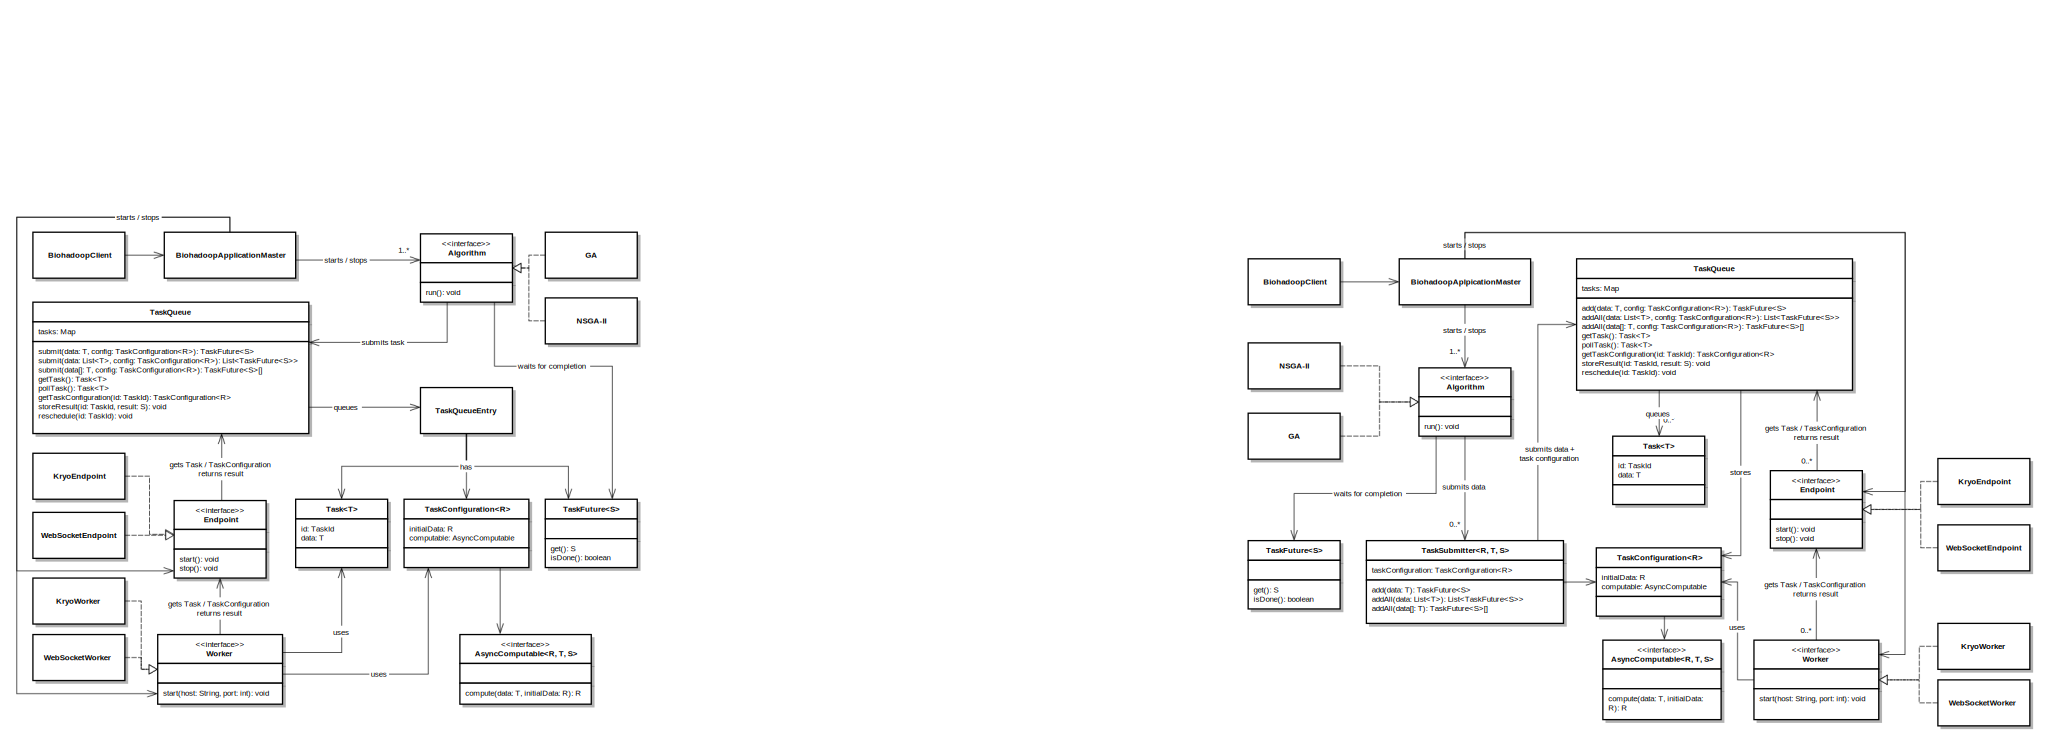
\includegraphics[width=140mm]{uml.png}
    \caption{Biohadoop UML Diagram}
    \label{fig:uml}
  \end{figure}
  
%   In addition, Figure \ref{fig:architecture} shows the architecture for offloading data from the main algorithm to local or remote workers. This is done by submitting chunks of data and a description of how to compute the results for this data chunks from the algorithm to the task system. In this architecture, the algorithm (section \ref{chap:impl:algorithm}) defines the problem that should be solved, e.g. an optimization problem. The data chunks, from here on called tasks, are smaller parts of this problem (e.g. compute the square root for a number), that can be submitted in an asynchronous fashion to the task system.
  
%   The task system consists of several parallel pipelines, whereas each pipeline is composed of task submitters, a task queue, adapters and workers. The tasks are actively requested by the workers, that communicate to their corresponding adapters. The adapters get the tasks out of the queues and deliver them to the workers. After the results are computed by the workers, those results are propagated back to the algorithm and the workers are free to request new tasks. The whole task system runs in an asynchronous fashion, submitted tasks are not blocking the algorithm. Section \ref{chap:impl:task-system} describes the task system in detail.\\
  
%   The task system relies on different communication mechanisms, to distribute the work among the waiting workers. Those communication mechanisms can be of any kind, whereas Biohadoop supports some types out of the box (local, HTTP, Kryo, Socket, Web Socket, as seen in figure \ref{fig:architecture}). The reason behind the decision to enable different kinds of communication mechanisms was, that all of them have different properties, and that for some workloads one may fit better then another. It is for example possible to distribute work to so called local workers. They are just threads and run inside the same JVM (Java Virtual Machine) as the algorithms, thus providing very little overhead to a solution that is implemented straight into the algorithm. By exposing a simple interface to the task system, changing later the type of worker (and with it the communication mechanism) to e.g. a remote type is just a matter of configuration. Another example would be when, during development, the socket communication is chosen. This is a performant way of communication, but may lead to firewall problems on some systems, as the right ports must be open. Changing this to use e.g. Web Sockets later on is, again, just a matter of configuration. More information about the communication mechanisms can be found in section \ref{chap:impl:communication}.\\


%  



% When an algorithm runs for a long time, it can be very annoying to lose results just because there was some kind of failure at any stage of computation. One solution to mitigate such problems is to save the current state of work to disk. Biohadoop supports its users in the task of saving and loading data with a set of classes and methods. One usage example is to reload the last state of an algorithm at startup, to continue the work at this point. To get more information about the persistence, refer to section \ref{chap:impl:persistence}.\\
%   
%   Biohadoop is capable of running several algorithms at the same time. They all run in the same JVM as Biohadoop does, and may be of the same type. As Hadoop on its own doesn't guarantee when a program runs, the mentioned capability of launching several algorithms at the same time in the same JVM is a useful enhancement when it comes to high level parallelization using the island model. If the algorithms were started by Hadoop one by one, it could be possible, that they were run in sequential order, instead of running at the same time.
%   
%   But Biohadoop doesn't restrict the usage of the island model to algorithms that run in the same JVM. By taking advantage of ZooKeeper \cite{zookeeper}, running algorithms may find each other also across the boundaries of different Biohadoop instances (Biohadoop can be started several times). This can lead to higher scalability, but entails the aforementioned problem, that Hadoop doesn't guarantee when a program runs, so a trade off has to be made. More information about how to use the island model in Biohadoop can be found in section \ref{chap:impl:island-model}\\
%   
%   To improve the understanding of the following sections, a simple example algorithm is introduced, called \texttt{Sum}. The algorithm takes an array of integers as input and provides the sum of them as result. For the sake of simplicity, we suppose that the input value of the \texttt{Sum} algorithm is never null. A simple implementation in Java can be found in listing \ref{listing:sum}, the output for different input values is given in table \ref{table:sum-algorithm}.
%   
%   \lstinputlisting[caption=Algorithm for integer summation,label=listing:sum]{../listings/chap4-sum.lst}
%   
%   \begin{table}
%     \centering
%     \setlength{\tabcolsep}{15pt}
%     \begin{tabular}{l|c}
%       numbers & sum \\ \hline
%       $[0]$ & $0$ \\
%       $[0,1]$ & $1$ \\
%       $[0,2,3]$ & $5$ \\
%     \end{tabular}
%     \caption{Example values for \texttt{Sum} algorithm}
%     \label{table:sum-algorithm}
%   \end{table}
% 
%   This example algorithm is good enough to demonstrate the usage of Biohadoop, other (more sophisticated) examples can be found at \cite{biohadoop-algorithms}. Chapter \ref{chap:usage} provides a step by step tutorial on how to implement this algorithm on Biohadoop.
%   
%   The following sections in this chapter continue to describe the implementation of Biohadoop in more detail, starting with the notion of Algorithm in section \ref{chap:impl:algorithm}. The next section \ref{chap:impl:task-system} talks about the task system, followed by the description of the communication mechanisms in section \ref{chap:impl:communication}. The enhancements section \ref{chap:impl:enhancements} talks about how Biohadoop supports persistence and the island model. How to configure Biohadoop is explained in section \ref{chap:impl:configuration}. If one just wants to use Biohadoop, chapter \ref{chap:usage} may be more helpful.
%   
% \section{Algorithm}
% \label{chap:impl:algorithm}
%   An algorithm in terms of Biohadoop is the implementation of an abstract problem that should be solved. For example, a genetic algorithm may be implemented to solve an optimization problem. Biohadoop supports the algorithm implementor with an easy way to parallelize the algorithm by providing an asynchronous task system (see \ref{chap:impl:task-system}). In addition, mechanisms for persistence and high level parallelization using an island model are offered (see \ref{chap:impl:enhancements}). All those capabilities can be used by the algorithm, but Biohadoop does not force their usage. The only thing an algorithm has to do to be run by Biohadoop, is to implement the \path{at.ac.uibk.dps.biohadoop.algorithm.Algorithm} interface, shown in listing \ref{listing:algorithm-interface}. This interface defines one method, which is invoked by Biohadoop after the system initialization has completed. There may run several algorithms of any kind at the same time in one Biohadoop instance, this is just a matter of configuration. After all algorithms have terminated, Biohadoop stops all components and shuts down.
% 
%   \lstinputlisting[caption=Algorithm interface,label=listing:algorithm-interface]{../listings/chap4-algorithm-interface.lst}
%   
%   \begin{itemize}
%     \item \texttt{void compute(SolverId solverId, Map<String, String>\newline configuration)}: This method is invoked by Biohadoop after the system initialization has completed. It is the place, where the algorithm should be implemented. The parameter \texttt{solverId} defines the global id of this instance of the algorithm, as there may run several instances of the same or different algorithms at the same time. The \texttt{solverId} can be used by other components to uniquely identify the algorithm. For example the persistence extension, which saves an algorithms state to a file, uses the \texttt{solverId} as part of the filename.
%     
%     The \texttt{properties} map contains the configuration for this algorithm (see \ref{chap:impl:configuration} for more information about how to configure Biohadoop). It is a map with key - value pairs of strings.
%     
%     The return value of the \texttt{compute} method is void, as there was no general return data identified, that could be useful. This may change in future versions.
%     
%     If there is an error during the algorithm execution, it may throw a  \path{at.ac.uibk.dps.biohadoop.algorithm.AlgorithmException} at any time. The meaning of a thrown \texttt{AlgorithmException} is, that there was an unrecoverable error which prevented the algorithm from progress, but the algorithm author was aware that such an error could happen, e.g. when a needed configuration argument is missing. Sometimes an algorithm may throw an unchecked exception, like the famous \texttt{NullPointerException}. The difference to \texttt{AlgorithmException} is in their semantics: unchecked exceptions are considered as the outcome of bugs. At the moment, Biohadoop makes no difference in handling \texttt{AlgorithmException} and unchecked exceptions, in both cases, the error is logged and the algorithm is terminated without affecting the other running algorithms. But it is possible that this behavior may change in the future. For example, it is thinkable that in the case of an \texttt{AlgorithmException}, a custom recovery procedure is invoked.
%   \end{itemize}
%   
%   When using the example algorithm from listing \ref{listing:sum}, without any further usage of the task system, persistence or high level parallelization, it would look like in listing \ref{listing:sum-biohadoop}. Note that there is no difference to the original implementation, except that now we have implemented the \texttt{compute(SolverId, Map<String, String>)} method.
%   
% 
%   \lstinputlisting[caption=\texttt{Sum} algorithm for integer summation on Biohadoop,label=listing:sum-biohadoop]{../listings/chap4-sum-biohadoop.lst}
% 
% \section{Task system}
% \label{chap:impl:task-system}
%   If an algorithm implementor decides to parallelize some parts of the algorithm, it can use Biohadoops task system. The task system works in an asynchronous manner and doesn't block its users while processing the tasks. However, it provides also mechanisms to block and wait for a result to be computed, if this is preferred.
%   
%   \subsection{Task pipeline}
%   \label{chap:impl:task-pipeline}
%   The task system is divided into several task pipelines, that run in parallel. Each pipeline has one or several task submitters, exactly one task queue, one or several adapters and one or several workers. Figure \ref{fig:single-pipeline} depicts the architecture of the task system with one task pipeline, consisting of one submitter, one queue, one adapter and one worker.
%   
%   \begin{figure}[ht!]
%     \centering
%     \includegraphics[width=130mm]{single-pipeline.png}
%     \caption{Task system with one task pipeline. The pipeline in this figure consists of one task submitter, one task queue, one adapter and one worker}
%     \label{fig:single-pipeline}
%   \end{figure}
%   
%   Central to each pipeline is the task queue. The queue is filled with tasks by the task submitters, that in turn get the tasks from the algorithm. Task submitters are a convenience abstraction that hide the complexity of task submission from the algorithm. An algorithm may choose to directly use a queue, although it is not recommended. Several submitters for one pipeline are supported.
%   
%   On the other side of the queue, we have the adapters and workers. The duty of the adapters is, to take tasks out of the queue and to pass them to the waiting workers, which do the (possibly heavy) computation of the tasks, and deliver the results back to the adapters. The adapters then propagate those results back to the algorithm. There may run several adapters and workers in each pipeline to enable parallel computation of the tasks. Each adapter can handle several workers.
%   
%   From the several parallel task pipelines, an algorithm can deliberately choose which one to use, it may use more then one. Figure \ref{fig:pipelines} for example depicts an algorithm, that uses four different task pipelines to handle its tasks, each pipeline consists of the before mentioned components. To enable the usage of several task pipelines in parallel and to distinguish them, unique names are used.
%   
%   \begin{figure}[ht!]
%     \centering
%     \includegraphics[width=130mm]{pipelines.png}
%     \caption{Several different named task pipelines may exist at the same time, consisting of submitters, queues, adapters and workers}
%     \label{fig:pipelines}
%   \end{figure}
% 
%   Every pipeline needs to be configured. To simplify this step, Biohadoop provides a pre-configured default pipeline, the \texttt{DEFAULT\_PIPELINE}. Using this default pipeline is advised, although it is possible to choose different pipelines for the task computation. Those other pipelines are from now on summarized under the term ``dedicated pipelines''. For example, the pipelines \texttt{PIPELINE\_A}, \texttt{PIPELINE\_B} and \texttt{PIPELINE\_C} in figure \ref{fig:pipelines} are dedicated pipelines, whereas the pipeline \texttt{DEFAULT\_PIPELINE} is the pre-configured default pipeline. All tasks submitted to the same pipeline share the same queue, adapters and workers.
%   
%   The main advantage of several parallel pipelines is better scalability. If one pipeline gets congested, a second pipeline, which works completely in parallel to the first one, can help to diminish this problem - given there are enough computational resources to effectively run the second pipeline. Another usage scenario for additional pipelines is, when there are tasks with different priorities, and one pipeline should only contain high priority tasks. By filling this pipeline only with high priority tasks, the tasks don't have to wait for other low priority tasks.
%   
%   The disadvantage of several pipelines is, that the workers of each pipeline receive only tasks from their pipeline. If no tasks are available (e.g. because there is not much work to do), then the workers have to wait, which can result in poor resource usage. Work stealing \cite{blumofe1999scheduling} between pipelines could reduce this problem, but is not implemented at the moment.
% 
%   Another disadvantage of dedicated pipelines is the slightly higher configuration effort, which really boils down to configure additional adapters and workers (more about this topic can be found in chapter \ref{chap:impl:configuration}, where the Biohadoop configuration is explained).
%   
%   In most cases, there is no need to run several pipelines and it is advised to start with the default pipeline. If there are good reasons, adding additional pipelines and dividing the tasks between them is straightforward.
%   
%   \subsection{Task Submitter}
%   \label{chap:impl:task-submitter}
%   The task submitter serves as the entry point to the task system and hides the complexity of the underlying components from the algorithm implementor. The generic interface \path{at.ac.uibk.dps.biohadoop.tasksystem.submitter.TaskSubmitter<T, S>}, shown in listing \ref{listing:taskSubmitter-interface}, defines the methods that a task submitter has to implement. T denotes the type of the task data, S denotes the type of the return value.
% 
%   \lstinputlisting[caption=TaskSubmitter interface,label=listing:taskSubmitter-interface]{../listings/chap4-taskSubmitter-interface.lst}
% 
%   \begin{itemize}
%     \item \texttt{TaskFuture<S> TaskSubmitter.add(T)}: This method adds a single task to a queue and returns a \texttt{TaskFuture}.
%     \item \texttt{List<TaskFuture<S>> TaskSubmitter.addAll(List<T>)}: This method adds a list of tasks to a queue and returns a list of \texttt{TaskFuture} objects, each one representing the result of exactly one submitted task. The tasks are then send one by one to the waiting workers.
%     \item \texttt{List<TaskFuture<S>> TaskSubmitter.addAll(T[])}: This method adds an array of tasks to a queue and returns a list of \texttt{TaskFuture} objects, each one representing the result of exactly one submitted task. The tasks are then send one by one to the waiting workers.
%   \end{itemize}
%   
%   \noindent
%   The methods of the \texttt{TaskSubmitter} interface return objects that implement \path{at.ac.uibk.dps.biohadoop.tasksystem.queue.TaskFuture<T>}, shown in listing \ref{listing:taskFuture-interface}, where T is the type of the return value. A \texttt{TaskFuture} object represents the result of an asynchronous computation performed by a worker, much like the \path{java.util.concurrent.Future} object, that is part of the Java standard.
% 
%   \lstinputlisting[caption=TaskFuture interface,label=listing:taskFuture-interface]{../listings/chap4-taskFuture-interface.lst}
% 
%   \begin{itemize}
%     \item \texttt{T get()}: Is used to wait until the result of a remote computation is available, which leads to a blocking behavior. After the result is available, \texttt{get()} returns this result.
%     \item \texttt{boolean isDone()}: Is used to check the task status, by which a non-blocking behavior can be realized. When \texttt{isDone()} returns true, the result can be obtained by invoking \texttt{get()} on the \texttt{TaskFuture} object.
%   \end{itemize}
% 
%   \noindent
%   The following code snippet illustrates a simple example, where a task is submitted to a queue, after which the program blocks until the result arrives by invoking \texttt{get()}. We assume here, that \texttt{taskSubmitter} is an initialized object that implements the \texttt{TaskSubmitter} interface. Further we assume, that the task data type is \texttt{String} and the return type is \texttt{int}:
%   \begin{lstlisting}
%     int result = taskSubmitter.add("Hello World!").get();
%   \end{lstlisting}
% 
%   The default implementation of the \texttt{TaskSubmitter} interface, that is provided by Biohadoop, is  \path{at.ac.uibk.dps.biohadoop.tasksystem.queue.SimpleTaskSubmitter}. It provides three different constructors that can be used to configure the details of task submission e.g. to which task pipeline a task is submitted. See listing \ref{listing:simpleTaskSubmitter} for more details about the constructors.
%   
%   \lstinputlisting[caption=SimpleTaskSubmitter,label=listing:simpleTaskSubmitter]{../listings/chap4-simpleTaskSubmitter.lst}
%   
%   As one can see, all constructors expect as parameter at least a class that extends the \path{at.ac.uibk.dps.biohadoop.tasksystem.AsyncComputable} interface. This class implements the part of the algorithm, that should be run on the workers and that is used to compute the results for the submitted tasks (more information about this interface and its usage can be found at section \ref{chap:impl:async-computable}).
%   
%   The second constructor expects an object containing the initial data, \texttt{initialData}, that should be available in the \texttt{AsyncComputable} class and therefore on the workers. This is suitable when several tasks need the same data for their computation, that doesn't change over time. The \texttt{initialData} is send to the workers when they first encounter a task that should be computed with a given \texttt{AsyncComputable} class. After that, this \texttt{initialData} is cached at the workers.
%   
%   For an example usage of the \texttt{initialData}, lets suppose we write an algorithm, that computes, for a list of locations, the distances to the nearest city and returns the nearest city. As input we have a list of cities with their coordinates (called \texttt{CITY\_LIST}), and a list of locations with their coordinates (called \texttt{LOCATION\_LIST}). This problem can be parallelized by breaking the list of locations down to single locations, for which the results can be computed in parallel. To get the nearest city for a given location, the algorithm computes the distances to all cities, and returns the city with the smallest distance. This algorithm could be implemented and parallelized with Biohadoop and its task system, where the task of computing the smallest distance for a given location is done by workers. Now, the \texttt{CITY\_LIST} remains the same for all locations, so it would be a bad idea to send the \texttt{CITY\_LIST} data to the workers for every task. This is the reason why the \texttt{initialData} exists: we set \texttt{CITY\_LIST} as initial data for the task submission and it gets transferred to a worker the first time it encounters this type of task (namely to compute the distance). After this first time, the \texttt{CITY\_LIST} can be reused by the worker, without the need to transmit it over and over. This usually results in much less overhead when the next task of this type has to be computed by the worker.
%   
%   The last constructor expects an additional \texttt{pipelineName} argument, that defines to which task pipeline the tasks, submitted using this task submitter, should be send. Using this constructor, an algorithm implementor is able to choose a dedicated pipeline for the task computation. Constructors that take no \texttt{pipelineName} argument, submit their tasks to the default pipeline.
%   
%   \subsection{Task Queue}
%   Tasks, submitted by the algorithms to be processed by the task system, are stored in task queues. The queue, where a task is stored, is part of the same pipeline as the task submitter, that put the task into the queue. There may exist several task queues, each queue is assigned to one task pipeline, which uses the queue exclusively during their whole lifetime. All tasks submitted to a given task queue have the same priority. Stored tasks are consumed by adapters and, from there on, handed to the workers for computation.
%   
%   Each task queue works as a first-in first-out (FIFO) queue. The head of the queue is that element, that has been on the queue the longest time. The tail of the queue is that element, that has been on the queue the shortest time. New elements are inserted at the tail of the queue. When reading from the queue, the head element is taken out of the queue and returned as result.
%   
%   Every task queue is backed by \path{java.util.concurrent.LinkedBlockingQueue}, which supports at maximum $2^{31} - 1$ number of elements, in this case tasks. The \texttt{LinkedBlockingQueue} supports concurrent addition and retrieval of elements. This facilitates the usage of many task submitters and adapters per queue. The \texttt{LinkedBlockingQueue} may block when adding an element and the queue is already full, or when an element should be taken out of an empty queue. In this two corner cases, also the task queue blocks. This may lead to the following problems:
%   \begin{itemize}
%     \item The task queue blocks when an algorithm wants to submit new tasks to a full queue. This kind of problem may arise if there is a huge number (more than $2^{31} - 1$) of tasks that are added to a task pipeline way faster than they can by computed. As a result, the algorithm gets also blocked and has to wait for free space in the task queue. This is a seldom case, but if it happens, there is the possibility to distribute the work between several task pipelines (and therefor between several queues), or to do the task submission in an own thread (could be implemented e.g. in a \texttt{TaskSubmitter}).
%     \item The task queue blocks, when an adapter wants to take a task out to send it to a waiting worker, but the queue is empty. This case happens often and results in blocking behavior of the adapters and workers. Adapters should therefor be prepared for this case and nevertheless at least accept new worker requests (Biohadoops provided adapters work in this manner). A way to diminish the blocking behavior would be to implement some kind of work stealing between queues, that is, an empty queue may fetch tasks from other queues that contain elements. This is not implemented at the moment. As a result, workers block if there is no work to do for their pipeline.
%   \end{itemize}
%   
%   As mentioned in the chapter before, it is preferable to submit tasks to a task queue by using the provided \path{at.ac.uibk.dps.biohadoop.tasksystem.queue.SimpleTaskSubmitter}, although it is not necessary. It is still possible to submit tasks directly to a task queue. To do this, first a reference to a task queue must be retrieved. This can be done by using the \texttt{at.ac.uibk.dps.biohadoop.tasksystem.queue.TaskQueueService}, which is a singleton and provides methods as seen in listing \ref{listing:taskQueueService}. Please keep in mind that the rest of this section is for advanced users only and may be skipped.
%   
%   \lstinputlisting[caption=TaskQueueService,label=listing:taskQueueService]{../listings/chap4-taskQueueService.lst}
%   
%   \begin{itemize}
%     \item \texttt{getInstance()}: is used to get an instance of the \texttt{TaskQueueService} singleton.
%     \item \texttt{TaskQueue<R, T, S> getTaskQueue(String name)}: this method provides a reference to a task queue with the given name. If no such task queue exists, a new one is created.
%     \item \texttt{stopAllTaskQueues()}: this method stops all task queues and should not be invoked by an algorithm implementor. It is used internally by Biohadoop in the shutdown process. When this method is called, all workers get notified to shut down. In addition, the task queue is removed from the internal storage and if there are no other references to this queue, it is made available for garbage collection.
%   \end{itemize}
% 
%   By invoking \texttt{getTaskQueue(String)} on the \texttt{TaskQueueService} singleton, a reference to a generic task queue is retrieved, which is of type \path{at.ac.uibk.dps.biohadoop.tasksystem.queue.TaskQueue}. The task queue offers the methods in listing \ref{listing:taskQueue}. The \texttt{add...()} methods are useful to submit new tasks, the  \texttt{stopQueue()} can be used to stop the queue and all of its depending workers. The other methods are usually used by adapters. When invoking the  \texttt{add...()} methods, new objects of type \path{at.ac.uibk.dps.biohadoop.tasksystem.queue.ClassNameWrappedTask} are created, that wrap the actual data, the information about which class to use to compute the result and a unique id. Those task objects can be retrieved by using the \texttt{getTask()} method.
%   
%   The generic types of the \texttt{TaskQueue} are T, which denotes the type of the task data, S denotes the type of the return value and R denotes the type of the inital data.
%   
%   \lstinputlisting[caption=TaskQueue,label=listing:taskQueue]{../listings/chap4-taskQueue.lst}
%   
%   \begin{itemize}
%     \item \texttt{add(T data, String asyncComputableClassName, R initialData) throws InterruptedException}: adds \texttt{data} of type T to the task queue, where \texttt{asyncComputableClassName} is the name of the class that should be used by the workers to compute this task. \texttt{initialData} is the data that is send to a worker when it first encounters this \texttt{asyncComputableClassName}. The method returns a \texttt{TaskFuture} object that represents the result of the computation (see chapter \ref{chap:impl:task-submitter} for more information about the \texttt{TaskFuture}). This method may throw an \texttt{InterruptedException}, if the underlying queue is interrupted while the task is inserted.
%     \item \texttt{addAll(List<T> datas, String asyncComputableClassName,\newline R initialData) throws InterruptedException}: adds a list of \texttt{datas} of type T to the task queue, where \texttt{asyncComputableClassName} is the name of the class that should be used by the workers to compute this tasks. \texttt{initialData} is the data that is send to a worker when it first encounters this \texttt{asyncComputableClassName}. The method returns a list of \texttt{TaskFuture} objects, each one representing the result of a computation. This method may throw an \texttt{InterruptedException}, if the underlying queue is interrupted while the task is inserted.
%     \item \texttt{addAll(T[] datas, String asyncComputableClassName,\newline R initialData) throws InterruptedException}:  adds an array of \texttt{datas} of type T to the task queue, where \texttt{asyncComputableClassName} is the name of the class that should be used by the workers to compute this tasks. \texttt{initialData} is the data that is send to a worker when it first encounters this \texttt{asyncComputableClassName}. The method returns a list of \texttt{TaskFuture} objects, each one representing the result of a computation. This method may throw an \texttt{InterruptedException}, if the underlying queue is interrupted while the task is inserted.
%     \item \texttt{getTask() throws InterruptedException}: gets the next \texttt{Task} object out of the task queue and returns it as result. This method may throw an \texttt{InterruptedException}, if the underlying queue is interrupted while the task is retrieved.
%     \item \texttt{getInitialData(TaskId taskId) throws TaskException}: this method gets the initial data for a task with the given \texttt{TaskId}. The \texttt{TaskId} is an internal id that is unique for every task. \texttt{Task} objects, that are returned by the \texttt{getTask()} method, encapsulate this \texttt{TaskId}.
%     \item \texttt{storeResult(TaskId taskId, S data)}: is used to store the result of the computation for the task with the given \texttt{TaskId}.
%     \item \texttt{reschedule(TaskId taskId) throws InterruptedException,\newline TaskException}: if something goes wrong while computing the result for a task, this task can be rescheduled, so it can be computed again. This method is useful e.g. in error conditions. It may throw an \texttt{InterruptedException}, if the underlying queue is interrupted while the task is inserted. It may throw a \texttt{TaskException} if the given \texttt{TaskId} is unknown to this task queue.
%     \item \texttt{stopQueue()}: stops this queue and notifies all workers to shut down.
%   \end{itemize}
% 
%   As one can see, the methods offered by the \texttt{TaskQueue} are rather low level. Direct usage of the \texttt{TaskQueue} is advised only if Biohadoop should be extended for example with new task submitters or new adapters.
%   
%   \subsection{Adapter}
%   \label{chap:impl:adapter}
%   An adapter takes tasks out of a queue and passes it to waiting workers through some kind of communication facility. The results returned by the workers are than handed back to the algorithm. So the most important aspect of an adapter is to communicate with the corresponding workers. This communication can be of any kind, and its technical details are hidden from an algorithm implementor. Already implemented examples for such communication types are HTTP, Kryo, Socket, WebSocket, but also simple variable sharing when the communication is done between different threads in the same JVM. Section \ref{chap:impl:communication} talks in greater detail about the communication aspects.
%   
%   As explained in the previous sections, there may be several task pipelines. Each pipeline consists of task submitters, a queue, the adapters and workers. Because of this rather tight coupling of queue, adapters and workers, adapters must be configured in a way, such that they know from which queue they should take the work. The default pipeline needs no configuration, for the configuration of a dedicated pipeline, take a look at section \ref{chap:impl:configuration}. There is no restriction on the number of running adapters.
%   
%   The communication types provided by Biohadoop should be enough for the average needs. But if one wants to use a different communication type, an implementation of the adapter and worker is needed. For the adapter side of the communication, this can be done through implementing the interface \path{at.ac.uibk.dps.biohadoop.tasksystem.adapter.Adapter}, shown in listing \ref{listing:adapter-interface}. Be aware that the methods in this interface are called by Biohadoop, so there is no need to call them somewhere manually, they are part of the life cycle of an adapter. This life cycle methods are called by Biohadoop in a sequential manner throughout all configured adapters, if one call blocks, the whole Biohadoop system blocks. The communication between adapter and workers is not part of this interface and can be designed as needed.
%   
%   Figure \ref{fig:flow-adapter} depicts the typical life cycle of an adapter. If any \texttt{configure(String)} or \texttt{start()} method throws an exception (in contrast to the figure), Biohadoop terminates at this point.
%   
%   \begin{figure}[ht!]
%     \centering
%     \includegraphics[width=130mm]{flow-adapter.png}
%     \caption{Life cycle of an adapter}
%     \label{fig:flow-adapter}
%   \end{figure}
%   
%   \lstinputlisting[caption=Adapter interface,label=listing:adapter-interface]{../listings/chap4-adapter-interface.lst}
% 
%   \begin{itemize}
%     \item \texttt{void configure(String pipelineName) throws AdapterException}: this method is called by Biohadoop when it prepares all the configured adapters. It provides a \texttt{pipelineName}, that defines the pipeline to which the adapter belongs. In addition, this is by convention the queue name, from which the adapter should consume the tasks. In this method, an adapter may initialize its behavior, but it should not start working (e.g. open a socket). It may throw a \texttt{AdapterException}, which leads Biohadoop to shutdown completely. Any other uncatched exception also leads to a complete shutdown. This is done to comply with the fail fast principle of application behavior \cite{shore2004fail}, which leads in this case to a system that is either running fully functional or not running at all.
%     \item \texttt{void start() throws AdapterException}: this method is called by Biohadoop to start all of the configured adapters. It is the right place to start up the adapters part of the communication, e.g. to open a listening socket. The method may throw a AdapterException which leads to a complete shutdown. Again, every uncatched exception also leads to a complete shutdown.
%     \item \texttt{void stop()}: This method is called by Biohadoop after all algorithms are finished, no matter if they threw an exception or not. In this method, the communication facility (e.g. socket) should be closed.
%   \end{itemize}
%   
%   \subsection{Worker}
%   \label{chap:impl:worker}
%   The workers implement the asynchronous (and possibly parallelized) part of the algorithm and actively request new tasks from the adapters. If the adapters have currently no work to offer, for example because the running algorithms have not submitted any tasks to the task system, then the workers wait until new work is available. Of course, the workers need some resources during the waiting times too (in terms of CPU, RAM, storage and so on), so when running Biohadoop, one should consider how much workers are really needed and at which point more of them are counterproductive.
%   
%   There are two different kinds of workers: the ones that run under the control of the Apache Hadoop system, (from now on called embedded workers) and the ones that run from outside of this system (from now on called external workers), Biohadoop supports both forms. Embedded workers must be configured in Biohadoop, but then the whole startup and shutdown is done automatically. In contrast, external workers don't have to be configured by Biohadoop, but their whole life cycle must be controlled in some other way, which is not part of Biohadoop. This can pose some problems, as external workers need to know e.g. when and where Biohadoop is running and how to connect to its running adapters. If there are no special needs, embedded workers are just fine. There are although some good reasons to use external workers:
%   
%   \begin{itemize}
%     \item external worker don't necessarily depend on the Hadoop ecosystem, they may run wherever they want, as long as they are able to communicate to at least one adapter. It is possible to develop external workers, that run in completely different environments for example mobile phones.
%     \item there is no restriction on the program language for an external worker, as long as it knows how to talk to at least one adapter. For example it is possible to implement a worker in JavaScript \cite{bioworker-browser} or Python \cite{bioworker-python}. In contrast to this, embedded workers have to be written in Java.
%     \item there is no limit in the number of external workers that may run. With suited algorithms to solve, this can lead to enormous scale. The algorithm should be suited in the sense, that the tasks are not to short running, as this would lead to high network traffic, effectively making this the bottleneck. The number of embedded workers is limited by the Hadoop environment, on which Biohadoop runs.
%   \end{itemize}
% 
%   Crucial to external workers is the fact, that they have to know how to communicate to the adapters. As it is not always easy to simulate e.g. the Java serialization mechanism in other languages, there are different kinds of adapters, that run different types of communication facilities. The most straight forward type of communication is using HTTP, a protocol for which there is an implementation in almost every language of the world. This way it is possible to implement external workers in a broad range of programming languages.\\
%   
%   
%   !!!!Workers don't get restarted if they fail!!!!\\
%   
%   
%   Embedded workers must implement the interface \path{at.ac.uibk.dps.biohadoop.tasksystem.worker.WorkerEndpoint}, that is shown in listing \ref{listing:worker-interface}.
% 
%   \lstinputlisting[caption=Worker interface,label=listing:worker-interface]{../listings/chap4-worker-interface.lst}
%   
%   \begin{itemize}
%     \item \texttt{String buildLaunchArguments(WorkerConfiguration\newline workerConfiguration) throws WorkerLaunchException}: this method is called by Biohadoop before the startup of the worker. The return value is a String, that contains needed configuration options for the worker to start. This string is provided to the worker at its startup. The reason for this method to exist is, that it is called inside the Biohadoop process, which opens the possibility to make use of Biohadoop internal configuration options and variables. After an embedded worker is started by Biohadoop (using the Hadoop YARN capabilities) it runs in a separated process on perhaps a different machine, and has no easy way to access the internal Biohadoop state. The method may throw a \texttt{WorkerLaunchException}, after which the whole Biohadoop system shuts down, in order to adhere to the fail fast principle. Every other uncatched exception also leads to the complete shutdown of Biohadoop.
%     \item \texttt{void configure(String[] args) throws WorkerException}: this method is called, after the embedded worker is instantiated i.e. when it is already running as a separate process on perhaps a different machine. The method takes an array of Strings as input parameters, which is exactly the array of Strings used to instantiate the worker process, or in other words, these are the parameters provided to the static \texttt{main(String args[])} method of the worker at startup. The arguments contain, beside the arguments of the \path{buildLaunchArguments(WorkerConfiguration)}, additional values, that may be useful, e.g. the path to Biohadoops config file. The method may throw a WorkerException, after which this worker is terminated and an error code of 1 is returned to Biohadoop.
%     \item \texttt{void start() throws WorkerException,\newline ConnectionRefusedException}: this method starts the main loop of the worker, where it begins to request tasks from the corresponding adapters. Usually, the adapter notifies the worker when to shutdown, which leads the worker to exit this method and to terminate its process with an exit code of 0. The method may throw a WorkerException after which this worker is terminated and an error code of 1 is returned to Biohadoop. It may throw a ConnectionRefusedException if it is unable to connect to its adapter. In this case, the worker shuts down, and an error code of 2 is returned to Biohadoop. Every other uncatched exception also shuts the worker down and returns an error code of 1 to Biohadoop.
%   \end{itemize}
%   
%   \begin{figure}[ht!]
%     \centering
%     \includegraphics[width=130mm]{flow-worker.png}
%     \caption{Life cycle of a worker}
%     \label{fig:flow-worker}
%   \end{figure}
%   
%   The typical life cycle of a worker is depicted in figure \ref{fig:flow-worker}. It begins at the Biohadoop instance, where the \texttt{buildLaunchArguments(\newline WorkerConfiguration)} method is called to get the necessary parameters. After that, Biohadoop launches for every worker instance a YARN container and starts the \texttt{at.ac.uibk.dps.biohadoop.tasksystem.worker.WorkerStarter} inside it. The \texttt{WorkerStarter} is responsible to call the \texttt{configure(String[] args)} and \texttt{start()} method of the worker. If an exception occurs, it is the responsibility of the \texttt{WorkerStarter} to terminate the work and return a corresponding exit value to Biohadoop. Please note, that figure \ref{fig:flow-worker} lacks information about the steps that are necessary to instrument the adapters. Information about those steps can be found in section \ref{chap:impl:adapter}.
%   
%   Inside the workers \texttt{start()} method, there is a main loop, where the worker asks for new tasks and submits the results of the computation to the adapters, which return them to the algorithm. The workers then wait for new tasks or for a shut down information from the adapters, which leads to its termination.
% 
%   By making the workers actively ask for new work, the adapters don't have to keep track of the workers. This way, the number of workers has no real limit. As long as a worker is able to connect to a corresponding adapter (where they have to agree on the protocol, communication flow and exchanged data, see section \ref{chap:impl:communication-flow} for more information), it may ask for work and return its results.
%   
%   !!!provide and describe implementation for AsyncComputable for Sum algorithm!!!
% 
%   \subsection{AsyncComputable}
%   \label{chap:impl:async-computable}
%   In the previous sections, the task system was introduced, but it wasn't mentioned, how the results for submitted tasks are computed. This is done, by defining classes that implement the generic interface \path{at.ac.uibk.dps.biohadoop.tasksystem.AsyncComputable<R, T, S>}. Each class that implements this interface declares, that it can be executed by workers. When an algorithm submits a new task, it has to define which \texttt{AsyncComputable} should be used for computing the result for the task. This information is then send, along with the task itself, to a worker, where the result is computed and then returned.
%   
%   In listing \ref{listing:asyncComputable-interface}, the method for the \texttt{AsyncComputable} interface is shown, where R is the type of the \texttt{initalData}, T is the type of input data and S is the type of the result.
%   
%   \lstinputlisting[caption=Classes that implement the AsyncComputable interface can be executed by workers,label=listing:asyncComputable-interface]{../listings/chap4-asyncComputable-interface.lst}
%   
%   \begin{itemize}
%     \item \texttt{S compute(T data, R initialData) throws ComputeException}: The code inside this method is executed by the worker. It gets \texttt{data} of type T and \texttt{initialData} of type S as arguments. The \texttt{data} represents the data for this task, \texttt{initialData} is some static data that doesn't change over time and that can be therefor cached by the workers, once they received it the first time. When the computation has finished, the result of type S is returned to an adapter and a new task is requested by the worker. The \texttt{compute(T, R)} method may throw a \texttt{ComputeException} at any time, indicating that something went wrong during the computation. This exception is logged by the workers, after that they terminate.
%   \end{itemize}
%   
%   \begin{figure}[ht!]
%     \centering
%     \includegraphics[width=130mm]{flow-asyncComputable.png}
%     \caption{Lifecycle of a task, computed by a worker using an AsyncComputable}
%     \label{fig:async-computable}
%   \end{figure}
%   
%   Figure \ref{fig:async-computable} depicts the general sequence of action for an asynchronous computation: a task is submitted to the task queue by an algorithm. As seen in section \ref{chap:impl:task-submitter}, this should be done using a \texttt{TaskSubmitter}. On submission, an \texttt{AsyncComputable} class must be declared, which is used by workers to compute the result for the task. At some point in time, an adapter takes the task out of the queue, together with the description of its related \texttt{AsyncComputable}. This step is triggered by an incoming worker request. The task, together with the description of its related \texttt{AsyncComputable}, is packed into a message and send to the requesting worker. On the worker side, the message is received and analyzed. Then, the result of the task is computed using an instance of the related \texttt{AsyncComputable}. The result is returned to the adapter and a new task is requested.
%   
%   There is one more step included, if the worker encounters an \texttt{AsyncComputable} that it hasn't seen before. In this case, the worker requests the \texttt{initialData} for this \texttt{AsyncComputable}, and only after it receives this data, it can proceed in computing the result of the task. The \texttt{initialData} should be cached by the worker, to minimize the communication overhead. All worker implementations provided by Biohadoop work this way.
%   
% \section{Communication}
% \label{chap:impl:communication}
%   In Biohadoop, algorithms can take usage of the task system to distribute their computation onto several waiting workers. As seen in the previous chapters, the task system consists of the submitters, a queue, adapters and workers. The submitters, queue and adapters all work in the same JVM and therefor in the same process. The communication between these parts is not difficult, it is just a matter of reading and writing shared variables between the different threads, possibly protected by concurrency protocols (for example, the queue is based on Java's \texttt{LinkedBlockingQueue}, which is a thread safe queue that supports many writers and readers).
%   
%   The communication between the adapters and workers is more complicated, as the adapters and workers may run in different processes, or even on different machines, so they can not rely on sharing variables between some threads. A more sophisticated method of communication must be used.
%   
%   There are many different ways of communication between different (remote) processes. Biohadoop provides five different communication protocols, that can be used to transfer the data between adapters and workers. The reason to not stick to just one implementation was, that each one has its advantages and disadvantages. As the whole communication process is hidden from the algorithm by the task system, changing the communication facility is just a matter of configuration, which makes it easy to try out different protocols and decide later on about which one to use.
%   
%   If there is the need for different, yet not implemented protocols, Biohadoop provides a way to implement its own protocols by implementing the appropriate parts of \texttt{Adapter} (section \ref{chap:impl:adapter}) and \texttt{Worker} (section \ref{chap:impl:worker}). The adapters and workers have to agree about the protocol, the serialization of the data and the communication flow.
%   
%   An introduction to the provided protocols is given in section \ref{chap:impl:protocols}. In section \ref{chap:impl:communication-flow}, the communication flow for the provided protocols is shown. It defines the steps involved for the communication between the adapters and the workers. Those steps are the same for all provided protocols. If one wants to implement its own communication mechanisms, it doesn't have to stick to the presented control flow and is free to choose its own one.
%   
%   \subsection{Protocols}
%   \label{chap:impl:protocols}
%     In this section, the five different communication protocols of Biohadoop are given, each one has its advantages and disadvantages.
% 
%     \subsubsection{HTTP}
%       Biohadoop provides an implementation of adapters and workers, that can communicate to each other by using HTTP. The adapter makes the tasks available as resources under a given URL. The URL is composed by the server name and port where the resource is available and the path \texttt{rs}, which is followed by the name of the task pipeline as subpath. For the default pipeline this would be for example \path{http://example.org/rs/DEFAULT_PIPELINE}. The workers take the tasks from this URL, compute the results and return those results to the same URL by using the \texttt{POST} verb.
%       
%       The main advantage of the HTTP protocol is, that it is in broad usage and that there exists an implementation for it in almost every language. This makes it very easy to write external workers in the desired language. The disadvantage of using HTTP is its speed, as there is a lot of overhead involved when sending HTTP requests over the wire (for example the HTTP headers).
% 
%       For serialization purposes, the JSON format is used. This is a very common format and suitable for machine communication, but also understandable for the human reader. Most programming language support JSON.
%     \subsubsection{Kryo and KryoNet}
%       Kryo \cite{kryo} is a library for high speed serialization of Java objects. It is usually faster than the build-in serialization features of Java. The developers of Kryo provide also the library KryoNet \cite{kryonet} for communication between different remote entities. This library is used by Biohadoop as one type of its provided protocols. The advantage consists of its speed, at least for the serialization.
%       
%       But as there where some problems when using KryoNet, the achieved communication speed is somewhat slower than with most of the other protocols. The problems are related to the asynchronous nature of KryoNet, where all requests are handled by exactly one event loop. If one request blocks (e.g. because it is waiting for new tasks), all other requests block too. To circumvent this, the requests are dispatched to special threads, but this slows the whole system noticeable down.
%       
%       Another disadvantage of Kryo and KryoNet is that they are custom serializers and protocol, that are not in broad usage. This restricts the worker implementations to be written in Java, which may not be a problem at all, especially if only embedded workers are used. But if external workers should be used, they have to be written in Java.
%       
%       Each class, that should be submitted between adapters and workers using Biohadoops Kryo protocol, must be registered with Kryo. The registration can be done by implementing the \path{at.ac.uibk.dps.biohadoop.utils.KryoRegistrator} interface in a registration object. This object then has to be made known to Biohadoop, by specifying its full class name in the \texttt{globalProperties} section of the configuration file (see section \ref{chap:impl:configuration} for more information about this topic). The name of the property must be \texttt{KRYO\_REGISTRATOR}. As an example, lets assume, that the full name of the configurator class is \path{com.biohadoop.KryoConfigurator}, then the property that needs to be set in the \texttt{globalProperties} section would be:
%       \begin{lstlisting}
% "KRYO_REGISTRATOR" : "com.biohadoop.KryoConfigurator"
%       \end{lstlisting}
%       When this parameter is set in the configuration file, Biohadoop knows that the classes, that are listed inside the configurator class, should be registered with Kryo.
%     \subsubsection{Socket}
%       When using the socket protocol, the communication and serialization is performed by the standard Java libraries. The communication is done using sockets, the serialization by the standard Java serializer. Each class, that should be submitted between adapters and workers using the socket protocol, must implement at least the \path{java.io.Serializable} marker interface. This is necessary for the standard Java serialization mechanism to succeed. As this serialization mechanisms can be somehow slow, there is the additional possibility, that a class implements the \path{java.io.Externalizable} interface, where the serialization has to be done manually.
%       
%       The advantage of the socket protocol is its very good performance, and that it is just a plain socket. Most languages provide mechanisms to connect to a socket, so this should be a rather easy task.
%       
%       The disadvantage of Biohadoops socket protocol is its dependence on the Java serialization, which restricts the workers to be written in Java or in a language that provides implementations for the Java serialization. This disadvantage may be mitigated by the possibility to implement a custom serialization mechanism by implementing the \texttt{Externalizable} interface.
%     \subsubsection{WebSocket}
%       WebSockets can be used for bidirectional communication. They were first used as an additional type of communication between a web application and an application server. They rely on the HTTP protocol for the handshake, during which the communication partners agree to upgrade to the WebSocket protocol. After the upgrade is done, the communication between the endpoints (in this case between the adapters and workers) can be performed using binary or text streams. Unlike in the plain HTTP protocol, the HTTP headers are not transmitted with every message, which reduces their size.
%       
%       Like in HTTP, the adapter makes the tasks available as resources under a given URL. The URL is composed by the server name and port where the resource is available, the path \texttt{ws}, which is followed by the name of the task pipeline as subpath. For the default pipeline this would be for example \path{http://example.org/ws/DEFAULT_PIPELINE}
%       
%       Unlike the HTTP protocol, for WebSockets there is no need to make a distinct request for every exchanged message. The worker just connects once to the URL and can then exchange all messages through this established connection.
% 
%       As already mentioned, the HTTP headers are omitted when WebSockets are used. This makes the data transfer faster than with HTTP, which is one of the advantages of using the WebSocket protocol in Biohadoop. Another advantage is, that WebSocket implementations are now available in many programming languages, making them available to a broad range of users, that may implement workers in their desired language. The disadvantage is that, if no WebSocket implementation exists in a language, it is harder to write a client, than e.g. for HTTP. Also, as WebSockets are a relatively new type of communication protocol, some available libraries may still contain bugs.
%       
%       JSON is used as the format for the data serialization, most languages provide parsers for it.
%     \subsubsection{Local}
%       The local communication can only be used with local workers. Those are workers, that run inside the same JVM (and therefor process) as Biohadoop and the algorithms. This makes it very easy to submit tasks and return results between adapters and workers. The data transfer is simply done by accessing shared variables. No serialization is needed, which greatly speeds up the communication between the adapters and workers. The access to the shared variables must be synchronized, as there may be several adapters and workers. This is done through standard Java mechanisms.
%       
%       The main advantage of the local protocol is its speed. As a process may use as much computational resources as available and because current hardware may provide a lot of shared CPU cores, the local protocol and workers may even scale to a sufficient degree for many tasks. But when greater scalability is needed, or when there are not enough computational resources available on the machine that runs Biohadoop, remote workers are needed, that rely on other communication protocols than the local one. Therefor the biggest disadvantage of local workers is, that they can run only on the local machine, where also Biohadoop runs.
%       
%   \subsection{Communication flow}
%   \label{chap:impl:communication-flow}
%     Each protocol presented in the prior section has to use some kind of communication flow between the corresponding adapters and workers. This communication flow, depicted in figure \ref{fig:communication-flow} is the same for all protocols that are provided by Biohadoop. If one wants to write a worker for one of the provided protocols, it must adhere to the communication flow presented here. Custom protocols don't need to reuse this, they are free to implement their own communication pattern.
%     
%     \begin{figure}[ht!]
%       \centering
%       \includegraphics[width=100mm]{communication-flow.png}
%       \caption{Communication flow}
%       \label{fig:communication-flow}
%     \end{figure}
%     
%     As one can see in figure \ref{fig:communication-flow}, the communication between adapters and workers is initialized by the worker. Also, after each iteration, the worker actively asks for new tasks.
%     
%     After the worker gets a task from the adapter, it has to control, if it already has the needed \texttt{initialData}. This is done by looking at the class name of the \texttt{AsyncComputable}, which is send along with the task. If the class is unknown, the worker asks the adapter for the \texttt{initialData} for the task. The adapter responds with the \texttt{initialData}, that is then cached by the worker, in case that the result for another task with the same \texttt{AsyncComputable} should be computed. Then, the worker computes the result for the task using the tasks data, the \texttt{AsyncComputable} and the \texttt{initialData}. The result is then retransmitted to the adapter and, at the same time, a new task is requested. Then the loop starts from the beginning.
%     
%     If the answer of the adapter consists of a shutdown message, the worker disconnects from the adapter and does the shutdown.
%     
%     The implementation of the presented communication flow has one big problem: a worker doesn't recognize when the same  \texttt{AsyncComputable} is used for different kinds of tasks with different \texttt{initialData} values. For example, lets assume that we have two different tasks, \texttt{TASK\_A} and \texttt{TASK\_B}. Each task uses the same \texttt{AsyncComputable} for its computation, but a different \texttt{initialData} value. Lets further assume, that a worker first encounters \texttt{TASK\_A}. In this moment, the worker will look up internally, if it has already the \texttt{initialData} for the \texttt{AsyncComputable}, that comes along with the task. In this case, this is not true, as the worker encounters this \texttt{AsyncComputable} the first time. The worker asks the adapter for the \texttt{initialData} and after its retrieval it stores this data internally. Then it computes the result for the task and returns it to the adapter. Now lets assume, that the worker gets next the \texttt{TASK\_B}. As the \texttt{AsyncComputable} is the same as for \texttt{TASK\_A}, and the worker looks up the \texttt{initialData} based on the \texttt{AsyncComputable}, the worker believes that it knows already the right \texttt{initialData}, which is wrong.
%     
%     This problem can be solved by transmitting a hash value of the \texttt{AsyncComputable} and \texttt{initialData}, in addition to the normal task data, and letting the worker decide, based on this hash, if it needs to fetch the \texttt{initialData}. This is not a big code change, and is on top of the TODO list for Biohadoop.
% 
% \section{Enhancements}
% \label{chap:impl:enhancements}
%   Beside the task system, that is presented in greater detail in section \ref{chap:impl:task-system}, Biohadoop provides two enhancements for algorithm authors. One is about persistence, where it is possible to load and store some data to disk (see section \ref{chap:impl:persistence}). The other is about high level parallelism between parallel running algorithms, called the ``iceland model'', that is sometimes used by optimization algorithms to enhance the solution (see section \ref{chap:impl:island-model}).
% 
%   \subsection{Persistence}
%   \label{chap:impl:persistence}
%   There are a lot of reasons for an algorithm to store its data to a disk. The most important may be, that one wants to store the result of a computation. The next reason is, to store the computational work that is done until a certain point, in case something happens. If this data can be reloaded afterwards, the computation can be continued from that point on. Another reason may be, that the intermediate results are needed for some other computation or visualization.
%   
%   So we see, that some kind of persistence is useful. It should include both the saving and loading of data. Biohadoop provides this kind of service by offering a simple API. Of course, an algorithm author may opt to use its own mechanism of data storage and retrieval, but the presented API has the advantage, that it is able to run both on local file systems and on Hadoops HDFS.
%   
%   The file saving is performed by using the class \path{at.ac.uibk.dps.biohadoop.persistence.FileSaver} and its provided static method, as presented in listing \ref{listing:chap4-persistence-save}.
%   
%   \lstinputlisting[caption=Save method exposed by \texttt{FileSaver},label=listing:chap4-persistence-save]{../listings/chap4-persistence-save.lst}
%   
%   \begin{itemize}
%     \item \texttt{static void save(SolverId solverId, Map<String, String>\newline properties, SolverData<?> solverData) throws\newline FileSaveException}: This method saves the data, provided by the \texttt{solverData} argument, to a file. The path for the file consists of the path that is defined in the configuration file under the algorithms private property with name \texttt{FILE\_SAVE\_PATH}, enhanced with the \texttt{solverId}. The filename consists again of the \texttt{solverId}, the iteration count that is submitted through the \texttt{SolverData} and the timestamp, at which the saving is done. The elements of the filename are separated by the character \texttt{\_}.
%     
%     So, for example, lets assume that the path defined in the configuration file is \path{/biohadoop/save}, the unique \texttt{solverId} is a UUID and has the value \path{08b1bc4c-e6d9-44ec-ba5d-24801f6c2339}, the iteration count is \text{100} and the timestamp, at which the saving is done, has the value \texttt{1411588421915}. Then the data, submitted with the \texttt{solverData} argument, is saved in the file:   
%     \begin{lstlisting}
% /biohadoop/save/08b1bc4c-e6d9-44ec-ba5d-24801f6c2339/08b1bc4c-e6d9-44ec-ba5d-24801f6c2339_100_1411588421915
%     \end{lstlisting}
%     
%     The saved data is stored in the file using the JSON format, which is a nice format for data serialization, that is available in many different programs, programming languages and environments.
%     
%     The method \texttt{save(SolverId, Map<String, String>, SolverData<?>)} throws a \texttt{FileSaveException} in the following cases:
%     \begin{itemize}
%       \item the \texttt{FILE\_SAVE\_PATH} property is not set
%       \item the save path can not be created
%       \item a file with the given name already exists
%       \item there was an error during the save operation
%     \end{itemize}
%     It is the responsibility of the algorithm author, to act appropriately to such an exception.
%   \end{itemize}
%   
%   As mentioned, the saving is configured in the configuration file. There are two properties, by which the saving can be adjusted to the personal needs (for more information about the configuration of Biohadoop, refer to section \ref{chap:impl:configuration}):
%   \begin{itemize}
%     \item FILE\_SAVE\_PATH: This is the initial path, where the files should be stored when they are saved. See the description of the \texttt{save(SolverId, Map<String, String>, SolverData<?>)} method above for more information about how the final file name is defined.
%     \item FILE\_SAVE\_AFTER\_ITERATION: Through this property, an algorithm author can decide after how many iterations a file should be saved. This removes from the algorithm author the burden of checking the iteration by hand. The \texttt{save} method than compares this value with the value that is provided in the \texttt{solverId} argument and decides, if it should persist the data.
%   \end{itemize}
%   
%   To load a file, for example to resume an old computation at the beginning of an algorithm, the class \path{at.ac.uibk.dps.biohadoop.persistence.FileLoader} can be used. This class provides a static method, presented in listing \ref{listing:chap4-persistence-load}.
%   
%   \lstinputlisting[caption=Load method exposed by \texttt{FileLoader},label=listing:chap4-persistence-load]{../listings/chap4-persistence-load.lst}
%   
%   \begin{itemize}
%     \item \texttt{static SolverData<?> load(SolverId solverId, Map<String, String>\newline properties) throws FileLoadException}: This method loads data from a file that is defined in the private property section of the algorithm under the name \texttt{FILE\_LOAD\_PATH}. This value can be defined in two ways. The first one defines the full path for a file, including the file name, that contains loadable data in a JSON format. In this case, exactly this file is loaded. In the second case, the value defines a directory path where loadable files can be found. In this case, the latest file in the directory is loaded, which is the file that was modified most recently. This can be suitable, when always the newest file of a directory should be loaded.
%     
%     The method throws a \texttt{FileLoadException} in the following cases:
%     \begin{itemize}
%       \item the \texttt{FILE\_LOAD\_PATH} property is not set
%       \item the file or path can not be found
%       \item the \texttt{FILE\_LOAD\_PATH} points to an empty directory
%       \item there was an error during the save operation
%     \end{itemize}
%     It is the responsibility of the algorithm author, to act appropriately to such an exception.
%   \end{itemize}
% 
%   Like in the case of file saving, the loading is configured in the configuration file. There are two properties, by which the loading can be adjusted to the personal needs:
%   \begin{itemize}
%     \item FILE\_LOAD\_PATH: This is the initial path, where the files should be stored when they are saved. See the description of the \texttt{save(SolverId, Map<String, String>, SolverData<?>)} method above for more information about how the final file name is defined.
%     \item FILE\_LOAD\_ON\_STARTUP: This boolean property defines, if the configured file should be loaded at all (the name is a bit confusing). If this property is not set, a call to \texttt{load} returns null as result. This can be convenient, if there is no useful data to load.
%   \end{itemize}
%   
%   \subsection{The island model}
%   \label{chap:impl:island-model}
%   The island model is a high level parallelization model, that is sometimes used in optimization problems. In the island model, there are several optimization algorithms running in parallel, trying to compute the result to the same problem. Those optimizers are called the islands. Each of these optimizers is independent of the others, and each one may have a different solution at a given point of time. By exchanging their data after some intervals, islands may get interesting solutions from other islands, that can be integrated in their own computation to enhance their solution.
%   
%   The island model greatly enhances the exploration behavior of optimizers, which often results in better overall solutions. As the data exchange is only done at certain points of time, the optimizers have the chance to exploit their own solution. When they get stuck in a local optima, they get the chance to escape this optima by getting another solution from another island.
%   
%     \subsubsection{API}
%     \label{chap:impl:island-model-api}
%     Biohadoop provides an API that can be used to build an island model. This API is exposed through the class \path{at.ac.uibk.dps.biohadoop.islandmodel.IslandModel} as seen in listing  \ref{listing:chap4-island-model}.
%     
%     \lstinputlisting[caption=Methods exposed by the \texttt{IslandModel} class. The class can be used to exchange data between the islands and therefor to construct an island model,label=listing:chap4-island-model]{../listings/chap4-island-model.lst}  
%     
%     \begin{itemize}
%       \item \texttt{static void initialize(SolverId solverId) throws\newline IslandModelException}: This method must be called by an algorithm to register it at the ZooKeeper service (see below for more information about ZooKeeper). It takes the \texttt{solutionId} as its only argument, which is the unique identifier for the algorithm.
%       
%       The method throws a \texttt{IslandModelException} if the host or port of ZooKeeper is not specified in the global properties of the configuration file. The host is specified through the \texttt{ZOOKEEPER\_HOSTNAME} property, the port through the \texttt{ZOOKEEPER\_PORT} property.
%       \item \texttt{static Object merge(SolverId solverId, Map<String, String>\newline properties, SolverData<?> solverData) throws\newline IslandModelException}: This method should be called, when the data merging should be done. The \texttt{solverId} identifies the algorithm, the \texttt{solverData} contains the current solution.
%       
%       The properties object is the map configured in the private property part of the algorithm. It uses strings for the keys and the values and must contain the following properties:
%       \begin{itemize}
% 	\item \texttt{ISLAND\_DATA\_REMOTE\_RESULT\_GETTER}: This property specifies a class that implements the interface \path{at.ac.uibk.dps.biohadoop.islandmodel.RemoteResultGetter} with the following method:
% 	\begin{lstlisting}
% Object getBestRemoteResult(List<NodeData> nodesData) throws IslandModelException
% 	\end{lstlisting}
% 	It has the job to get an appropriate remote result from a remote island. To perform this job, a list of \texttt{NodeData} elements is provided, that represents all currently known islands. From this list, a suitable solution should be chosen and returned.
% 	\item \texttt{ISLAND\_DATA\_MERGER}: This property specifies a class that implements the merging of the local and a remote solution. This class must implement the generic \path{at.ac.uibk.dps.biohadoop.islandmodel.DataMerger} interface with the following method, where T is the generic type:
% 	\begin{lstlisting}
% T merge(T o1, T o2)
% 	\end{lstlisting}      
% 	The job of this method is to merge the data of the solutions given as \texttt{o1} and \texttt{o2} into a new solution.
%       \end{itemize}
%       
%       The \texttt{merge(SolverId, Map<String, String>, SolverData<?>)} method throws an \texttt{IslandModelException} at the same conditions as the \texttt{initialize(SolverId)} method mentioned above. In addition, it throws the \texttt{IslandModelException} if the \texttt{RemoteResultGetter} or the \texttt{DataMerger} classes are not defined or can not be instantiated. Also, the \texttt{RemoteResultGetter} or the \texttt{DataMerger} may throw this exception, if there is something wrong during the data merging. It is the responsibility of the algorithm author, to act appropriately to such an exception.
%     \end{itemize}
%     
%     To make its own solution available to other islands, the data must be explicitly set by the algorithm author. This is done by using the following method of the \path{at.ac.uibk.dps.biohadoop.datastore.DataClient} object:
%     \begin{lstlisting}
% static <T> void setData(SolverId solverId, Option<T> option, T data)
%     \end{lstlisting}   
%     
%     It takes as arguments the \texttt{solverId}, the second argument in this case must be \path{DataOptions.SOLVER_DATA}, and the third argument should be the data, wrapped in a \path{at.ac.uibk.dps.biohadoop.solver.SolverData} object.
% 
%     \subsubsection{ZooKeeper}
%     \label{chap:impl:island-model-zookeeper}
%     As mentioned above, Biohadoops island model API takes usage of ZooKeeper \cite{zookeeper}, which is a Server that provides distributed configuration and synchronization services, and a naming registry. Therefor, a running ZooKeeper instance must be accessible by Biohadoop.
%     
%     When using the island model, the algorithms first have to register to ZooKeeper by using the \texttt{initialize(SolverId)} method of the \texttt{IslandModel}. The registration adds an entry to ZooKeeper, that is visible to all other algorithms that use the island model API. The path to the registration is defined by the fixed string \path{/biohadoop/solvers}, followed by the simple class name of the algorithm and the \texttt{solverId} as subpath. For example lets assume that the full class name of our algorithm is \path{org.example.Sum} and that its \texttt{solverId} is \texttt{08b1bc4c-e6d9-44ec-ba5d-24801f6c2339}. Then the path, at which the algorithm registers itself to ZooKeeper is
%     \begin{lstlisting}
% /biohadoop/solvers/Sum/08b1bc4c-e6d9-44ec-ba5d-24801f6c2339
%     \end{lstlisting}
%     
%     The registration data consists, again, of the \texttt{solverId} and a URL, where the current solution for the algorithm can be found, both serialized using the JSON format. An example for this data can be found in listing \ref{listing:chap4-zookeeper-registration-data}, where the relevant information is on line 1.
%     
%     \lstinputlisting[caption=Example for ZooKeeper registration data,label=listing:chap4-zookeeper-registration-data]{../listings/chap4-zookeeper-registration-data.lst}
%       
%     When the data merging between islands should be done, the defined \texttt{RemoteResultGetter} gets a list of all the algorithms that are registered at ZooKeeper, along with their registration data. With this information, that contains also the URL where the current solution for the islands can be found, the \texttt{RemoteResultGetter} chooses which remote solution should be used for the subsequent merge.
%     
%     The remote solutions are made available as HTTP resources at the URL that is part of the registration information, where the complete URL consists of the URL from the ZooKeeper registration with the \texttt{solverId} appended, for example:
%     
%     \begin{lstlisting}
% http://example.org:30000/rs/islandmodel/08b1bc4c-e6d9-44ec-ba5d-24801f6c2339
%     \end{lstlisting}  
%     
%     In the end, the whole process of registration to ZooKeeper, retrieval of this information from ZooKeeper and publishing the result of the computation at a defined URL is done by the island model API behind the curtains, so an algorithm author doesn't have to bother with it. The only things an algorithm author has to do is to
%     \begin{itemize}
%       \item provide its data using the \texttt{DataClient.setData(SolverId, Option<T>, T)} method
%       \item use the provided methods of the \texttt{IslandModel} object when the merging should be done
%       \item provide an implementation of \texttt{RemoteResultGetter} and \texttt{DataMerger} to define which data should be merged and how the merging should be done
%     \end{itemize}
% 
%     By using ZooKeeper as central registry for the island model, and by exchanging the data between the islands through HTTP, it doesn't matter if the algorithms run in the same Biohadoop instance (which is possible by defining several instances in Biohadoops configuration file), or if the algorithms run in different Biohadoop instances. The only advantage of running several algorithms in the same Biohadoop instance is, that it guarantees that they all run at the same time. When running several Biohadoop instances on Hadoop, it isn't guaranteed that they also run at the same time, as Hadoop decides when to launch a program. If the algorithms don't run at the same time, then there is no data exchange possible between them, so the island model is reduced to one single island, which means that it makes no difference to running the algorithm without the island model.
%   
% \section{Configuration}
% \label{chap:impl:configuration}
%   Biohadoop uses a configuration file in JSON format. This has the advantage, that it isn't hard for humans to understand and modify its content. It usually is also smaller in size than e.g. XML and parsers exist for a broad range of programming languages. To provide support for automatic schema validation, JSON Schema \cite{json-schema} is used. The full JSON Schema \cite{json-schema} for the configuration file can be found in the appendix \ref{lst:json-schema}.
%   
%   The path to the configuration file must be given on invocation of Biohadoop as its first parameter (more information on how to run Biohadoop can be found in \ref{chap:usage:run}). If the path is empty or wrong, Biohadoop stops immediately with an \texttt{IllegalArgumentException}. If a file is found, its content is parsed and Biohadoop tries to build a configuration object out of it. If there was an error during parsing, Biohadoop stops with an \texttt{IOException}, \texttt{JsonParseException} or \texttt{JsonMappingException}, depending on the reason of the error. Supposing everything went right, the configuration is exposed through the static class \path{at.ac.uibk.dps.biohadoop.hadoop.Environment} and its \texttt{getBiohadoopConfiguration()} method.
%   
%   Note that the exposure is restricted to the JVM that runs Biohadoop. But this should be enough for most purposes. The algorithms can directly access the \texttt{Environment}, although this should be seldom necessary, as the algorithm get their parameters as arguments. Adapters are also able to access the \texttt{Environment}. Both mentioned components run in the same JVM as Biohadoop does.
%   
%   When it comes to the workers and the \texttt{AsyncComputable} methods that they run, things are a little bit different. The workers run on different JVMs than Biohadoop does (except the local running workers, that run as separate threads), so they don't have direct access to the \texttt{Environment} object. Nevertheless, the path to the configuration file is provided also to the workers, such that they could read and parse the configuration file. But at the time of this writing, there was no reason for a worker or \texttt{AsyncComputable} to access the configuration file directly, therefor the access is currently not implemented. Changing this at a later stage is not a big task.
%   
%   The configuration file itself consists of the following four top-level objects:
%   \begin{itemize}
%     \item \texttt{communicationConfiguration}: defines lists for additional adapters and all workers, that Biohadoop should start. Additional in the sense, that adapters for dedicated pipelines must be configured right here, whereas adapters for the default pipeline don't have to be configured. The workers must be also defined here, for all pipelines including the default pipeline, since there is no useful default configuration for workers. 
%     \begin{itemize}
%        \item \texttt{dedicatedAdapters}: a list of additional adapters. Each element in the list is of type \path{at.ac.uibk.dps.biohadoop.tasksystem.adapter.AdapterConfiguration}, that contains the canonical class name of an \texttt{Adapter} and a string that defines to which pipeline that adapter belongs.
%        \begin{itemize}
%          \item \texttt{adapter}: canonical class name of the \texttt{Adapter}
%          \item \texttt{pipelineName}: string that defines to which pipeline that adapter belongs
%        \end{itemize}
%        \item \texttt{workerConfigurations}: a list of workers: Each element in the worker list is of type \path{at.ac.uibk.dps.biohadoop.tasksystem.worker.WorkerConfiguration}, that contains the canonical class name of a \texttt{Worker}, a string that defines to which pipeline that worker belongs and a counter that indicates how many instances of this worker should be started.
%        \begin{itemize}
%          \item \texttt{worker}: canonical class name of the \texttt{Worker}
%          \item \texttt{pipelineName}: string that defines to which pipeline that worker belongs
%          \item \texttt{count}: number of instances of this worker
%        \end{itemize}
%     \end{itemize}
%     \item \texttt{globalProperties}: a map with strings as keys and values. This properties are used for global settings, that should be available in different places.
%     \item \texttt{includePaths}: a list of strings that define the paths where needed libraries can be found. This isn't important for a local running instance of Biohadoop (e.g. during development), as the necessary classpaths must be set when starting Biohadoop. But it is important when Biohadoop runs in the Hadoop environment, as this are the paths with libraries, that Hadoop should provide to Biohadoop when running. If the paths to the necessary libraries are not set correctly when running on Hadoop, \texttt{ClassNotFoundException} are thrown.
%     \item \texttt{solverConfiguration}: a list of algorithms that should be run by Biohadoop. Each element in the list is of type \path{at.ac.uibk.dps.biohadoop.solver.SolverConfiguration}, that contains the canonical class name of an \texttt{Algorithm}, a freely selectable name for it, and a map of properties, that are passed to the algorithm as argument.
%     \begin{itemize}
%       \item \texttt{algorithm}: canonical class name of the \texttt{Algorithm}
%       \item \texttt{name}: freely selectable name, is shown for example in the log files
%       \item \texttt{properties}: a map with strings as keys and values. This properties are used for this instance of the algorithm and should be considered private to it. This properties are provided as second argument to the algorithm, when its \texttt{compute(SolverId, Map<String, String>)} method is invoked.
%     \end{itemize}
%   \end{itemize}
% 
%   Listing \ref{lst:sum-configuration} illustrates a very simple configuration file for the \texttt{Sum} algorithm, introduced in section \ref{chap:impl:system-architecture}. The implementation can be found in \cite{biohadoop-algorithms}. The algorithm sums up all values of an integer array. It takes as input arguments the the number of chunks (\texttt{CHUNCKS}) of integer arrays. As second input argument it takes the size of each chunk (\texttt{CHUNCK\_SIZE}). The whole integer array has then the size $\texttt{CHUNCKS} * \texttt{CHUNCK\_SIZE}$. The chunks are submitted to the task system, the sum for each chunk is computed on workers and then returned back to the algorithm, where the final summation for all chunks is done.
% 
%   \lstinputlisting[caption=Simple configuration file for the \texttt{Sum} algorithm\, introduced in section \ref{chap:impl:system-architecture},label=lst:sum-configuration]{../listings/chap4-sum-configuration.lst}
%   
%   At line 2 we have the configuration of the paths, that have to be included when running Biohadoop. This setting is only important if Biohadoop runs in a Hadoop environment. It is not important if it runs in local mode, for example during development. When running on Hadoop, the files in this directories are made available to Biohadoop.
%   
%   At line 3 starts the communication configuration, which consists of a list of dedicated adapters and a list of all workers. The definition of dedicated adapters at line 4 is empty, as \texttt{Sum} uses only the default pipeline for computation. If dedicated pipelines were used, than the adapters for this pipeline must be configured here.
%   
%   Beginning with line 5 we have the declaration of the workers, that Biohadoop should launch. Each entry is defined by the a worker class name, a pipeline to which this worker is assigned, and the number of workers of this instance, that should be launched. We see here for example, that 5 workers of different types are configured, but only the \texttt{LocalWorker} at line 10 should be instantiated once. All other workers have a count of 0, which means that no instances of these workers are launched.
%   
%   At line 27 we have the definition of the global properties. Again, \texttt{Sum} doesn't take usage of this configuration possibility. Other algorithms instead use this place for example to specify the configuration for ZooKeeper.
%   
%   At line 28, the definition for the algorithm starts. In this case, only one algorithm should be started, it is the algorithm with class \texttt{SumAlgorithm}. The name of the algorithm is \texttt{SUM}, which can be seen e.g. in the log output of Biohadoop. At line 31 there is the configuration of the properties, that are submitted to the \texttt{compute(SolverId, Map<String, String>)} method of the algorithm. Those are the properties described before (\texttt{CHUNCKS} and \texttt{CHUNCK\_SIZE}).
%  
%   It is not always convenient to write the configuration for an algorithm by hand, although it is possible. Biohadoop provides two builder classes, to make it more easy to produce config files. The builder in \path{at.ac.uibk.dps.biohadoop.hadoop.BiohadoopConfiguration} offers methods to configure the top level elements of a configuration file (\texttt{communicationConfiguration}, \texttt{globalProperties}, \texttt{includePaths}, \texttt{solverConfigurations}). The configuration for solvers is simplified by the builder in \path{at.ac.uibk.dps.biohadoop.solver.SolverConfiguration}. The result of this solver configuration can then be handed over to the \texttt{BiohadoopConfiguration} builder. Listing \ref{lst:sum-configuration-builder} shows how the configuration for the \texttt{Sum} algorithm can be performed by using the mentioned builders. Note that the outcome of this listing is exactly the config file of listing \ref{lst:sum-configuration}.
%   
%   \lstinputlisting[caption=Example on how to produce a configuration file for the \texttt{Sum} algorithm\, using the provided builders. The output of this program can be found in listing \ref{lst:sum-configuration},label=lst:sum-configuration-builder]{../listings/chap4-sum-configuration-builder.lst}
%   
% \section{BioOozie}
% \label{chap:impl:oozie}
%   \begin{itemize}
%     \item where fits oozie in the picture?
%     \item advantage of using oozie / problems with oozie (not guaranteed that oozie starts parallel task in parallel)
%     \item custom tag / extension
%     \item configuration / why using json rather than XML
%     \item extension possibilities (extend tags in a way that XML configuration can be submitted to biohadoop (e.g. make json out of xml configuration, save to file, start biohadoop))
%   \end{itemize}
% %%%% DELETABLE!!!!

\chapter{Using Biohadoop}
\label{chap:usage}
One of the design goals of Biohadoop was to provide a framework for distributed computation on the Hadoop platform, that is easy to use. The result is a simple API, that can be used to implement algorithms. This chapter introduces into the necessary steps to write an algorithm that is capable of being run by Biohadoop on a Hadoop environment. In addition, the presented algorithm uses the capabilities of the task system to distribute parts of its work to Biohadoops workers, to achieve a higher level of parallelism.

% \section{Example algorithm}
% \label{chap:usage:algorithm}
% For the sake of simplicity we reuse the example algorithm \texttt{Sum} of chapter \ref{chap:impl:system-architecture}. As mentioned there, it is a simple algorithm, whose only purpose is to sum the values of an integer array. In listing \ref{listing:sum} we have already a first implementation, that is capable of being run by Biohadoop. But in that example, no usage of the task system and therefor distribution is taken. Also, all the parameters are fixed. In the next sections, we will create step by step an implementation that is configurable using Biohadoops configuration file, and that is able to distribute its work (see section \ref{chap:impl:configuration} for more details about the configuration file).
% 
% To make it more transparent how and when we use the task system, we modify the algorithm a little bit. It should use a number of integer arrays (the number is called \texttt{CHUNKS} from here on), each array should be of a fixed size (the size is called \texttt{CHUNK\_SIZE} from here on). If we would append all the chunks one after another, we would have one big integer array of size $\texttt{CHUNCKS} * \texttt{CHUNCK\_SIZE}$. If you look at it from the other side, a big integer array would have to be split into several chunks, to make it suitable for parallel computation. So there is no real difference to the original algorithm, it just preserves us from doing some computations to split a big integer array into smaller arrays. 
% 
% Listing \ref{lst:usage-build-data} shows how the data is created. The method \texttt{buildData(int chunks, int chunkSize)} takes \texttt{CHUNCKS} and \texttt{CHUNCK\_SIZE} as input argument and returns \texttt{CHUNKS} integer arrays, each of size \texttt{CHUNCK\_SIZE}. The arrays are filled with consecutive numbers, starting from 0. The consecutive numbers continue between the boundaries of adjacent arrays. For example, array0=[0,1,2], array1=[3,4,5], ...
% 
% \lstinputlisting[caption=Building the integer arrays for the \texttt{Sum} algorithm,label=lst:usage-build-data]{../listings/chap-usage-buildData.lst}
% 
%   \subsection{Configuring the algorithm}
%   \label{chap:usage:configuration}
%   Lets begin with modifying the algorithm in a way, such that it can be configured by Biohadoops configuration file. The configuration file is read by Biohadoop at its startup, and the private parameters for an algorithm instance are provided when the \texttt{compute(SolverId solverId, Map<String, String> properties)} method of the algorithm is called. If we use the configuration file of listing \ref{lst:sum-configuration}, we see that we get two properties:
%   \begin{itemize}
%     \item \texttt{CHUNKS}: the number of integer arrays, that should be produced by the algorithm.
%     \item \texttt{CHUNK\_SIZE}: the size of each integer array.
%   \end{itemize}
%   Those parameters are of type \texttt{String}, so we need to convert them first to integer values, to make them suitable for the \texttt{buildData(int, int)} method, mentioned in listing \ref{lst:usage-build-data}. After this steps are taken, we have configured our algorithm through a Biohadoop configuration file, and we have initialized the data. Listing \ref{lst:usage-configured} shows, how the algorithm looks at the current stage. The \texttt{buildData(int, int)} method was skipped, to make the code more concise, it can be found in listing \ref{lst:usage-build-data}.
%   
%   \lstinputlisting[caption=Configuring the \texttt{Sum} algorithm and initializing the data,label=lst:usage-configured]{../listings/chap-usage-configured.lst}
% 
%   \subsection{Parallelization using the task system}
%   \label{chap:usage:parallel-algorithm}
%   The parallelization of an algorithm using Biohadoop consists of four steps:
%   \begin{enumerate}
%     \item provide an implementation of \texttt{AsyncComputable}, that can be used to compute the task results by the workers.
%     \item create a task submitter, that can be used to add new tasks to the task system.
%     \item submit tasks to the task system, by using the before mentioned submitter.
%     \item wait for the tasks to complete. It is possible to block during the wait process, but is also possible to do other work in between.
%   \end{enumerate}
%   
%   In step 1 we have to implement \texttt{AsyncComputable}. The resulting class can be used by the workers to compute the results for the tasks. In our case, the workers get as input arguments an integer array and have to compute the sum over all of its elements. Listing \ref{lst:usage-async-computable} shows how this would be done in a class with name \texttt{AsyncSumComputation}. We see that this class is typed, the types have to match the task submitter in step 2. The types are \texttt{Object} for the \texttt{initialData}, but we don't take usage of it in this case. The input data is of type \texttt{int[]}, which matches our integer arrays. As output we have a single integer, which is the result of the summation. The content of the method itself is straight forward.
%   
%   \lstinputlisting[caption=Summation of all values in an integer array\, done in an \texttt{AsyncComputable} class\, that is suitable to be run by workers,label=lst:usage-async-computable]{../listings/chap-usage-asyncComputable.lst}
%   
%   Step 2 demands the creation of a task submitter, to be able to add tasks to the task system. Lets clarify at this point, what a single task means in our example program: each single task consists of computing the sum of an integer array. The data for this task is the given integer array. This data is send to workers, that use a given \texttt{AsynComputable} class to compute the result - in our case the sum of the integer array computed by the \texttt{AsyncSumComputation} class. The result is then returned to the algorithm, at which point the task has completed.
%   
%   The \texttt{Sum} example algorithm uses many integer arrays, therefor we have many tasks, one task for every integer array. Tasks are submitted to the task system, by submitting their data through a task submitter. The usage of a task submitter is advised, as it hides some complexity from the algorithm author. But it is possible to communicate to the task system without a submitter. We choose to use the task submitter, and create a new one the following way:
%   
%   \begin{lstlisting}
% TaskSubmitter<int[], Integer> taskSubmitter = new SimpleTaskSubmitter<Object, int[], Integer>(AsyncSumComputation.class);
%   \end{lstlisting}
%   
%   This task submitter is configured to get an object of type \texttt{Object} as \texttt{initialData}. As we don't want to use this feature, we don't provide such an \texttt{initialData}. The submitter is further configured to receive tasks of type \texttt{int[]} and to return \texttt{TaskFutures} of type {Integer}, that can be used by the algorithm to retrieve the results from the task system. The tasks of type \texttt{int[]} that we are going to submit are exactly the arrays, that we created in the previous section, using the \texttt{buildData(int, int)}. We store all those arrays in a single 2-dimensional array of type \texttt{int[][]} and call this array \texttt{data}. The only parameter that we provide to the new instance of \texttt{SimpleTaskSubmitter} is the \texttt{AsyncSumComputation} class. This class is used by the workers to compute the results for the tasks, that are submitted through this task submitter.
% 
%   In step 3 we start to submit tasks to the task system. As we want to submit a number of arrays, it is best to do it in a loop. We also want to be able to use the results of the different sums to compute the final sum. Therefor we have to store the \texttt{TaskFutures}, to be able to retrieve their results:
%   
%   \begin{lstlisting}
% List<TaskFuture<Integer>> taskFutures = new ArrayList<>();
% for (int i = 0; i < chunks; i++) {
%   TaskFuture<Integer> future = taskSubmitter.add(data[i]);
%   taskFutures.add(future);
% }
%   \end{lstlisting}
%   
%   Step 4 consists of waiting for the results. The \texttt{get()} method of a \texttt{TaskFuture} provides us the result, but blocks until a result is available. \texttt{TaskFuture} provides also a \texttt{isDone()} method, which we can use to check for finished computations in a non-blocking way. If \texttt{isDone()} returns true, we can get the results by invoking \texttt{get()}, that doesn't block anymore at that time.
%   
%   We choose the simpler \texttt{get()} approach at the cost of blocking the algorithm. As we need all results to proceed, this makes no difference to the non-blocking variant. Because we got several \texttt{TaskFuture} objects from our task submissions in step 3, we have to loop on all the \texttt{TaskFuture} objects to get all of their results. By summing up the results, we get the final sum over all arrays:
%   
%   \begin{lstlisting}
% int sum = 0;
% for (TaskFuture<Integer> future : taskFutures) {
%   sum += future.get();
% }
%   \end{lstlisting}
%   
%   After this step completes, we have the final sum over all arrays, and the algorithm can terminate.
%   
%   Something that wasn't mentioned until now is, that the task submission and result retrieval operations may throw checked exceptions. This exceptions must be caught, therefor the submission and retrieval must be surrounded by a \texttt{try ... catch} block. In the example code above, this step was omitted to keep the code clear and concise. In the appendix, the whole code can be found, once for the \texttt{Algorithm} (see listing \ref{lst:appendix-sum-full}), and once for the \texttt{AsyncComputable} (see listing \ref{lst:appendix-sum-async}). More examples can be found at \cite{biohadoop-algorithms}.
  
\section{Run Biohadoop}
\label{chap:usage:run}
Although the main purpose of Biohadoop is to be run in a Hadoop environment, it can also be run in a local environment. This is for example useful when new algorithms are developed. In this case, the whole process of compilation, deployment to a Hadoop environment and testing can be abbreviated.

To run Biohadoop, three components must be available (four if Biohadoop is started in a Hadoop environment):

\begin{itemize}
  \item An installation of Java in version 1.7 or higher. From here on it is assumed, that Java is installed and configured and that the \texttt{JAVA\_HOME} variable points to this installation.
  \item All necessary libraries must be present and accessible in one or several folders.
  \item A valid configuration file must be present and accessible.
  \item The fourth component is only necessary when running Biohadoop in a Hadoop environment. This component is Hadoop itself, which must be available in a version $\geq 2$.
\end{itemize}

If those three components are provided (four for running on Hadoop), Biohadoop can be started. In a local environment, this is done by setting the right class paths when launching the program. In a Hadoop environment, the configuration option \texttt{includePaths} must be set, to include the necessary files (see \ref{chap:impl:configuration} on more information about configuring Biohadoop). Those paths have to point to valid locations of an accessible HDFS file system.

Biohadoop was developed using Maven. \footnote{\url{http://maven.apache.org/} last access: 11.09.2014} Therefor it is rather easy to get all the needed libraries, as they are declared as dependencies. The source code for Biohadoop can be found at \cite{biohadoop}. By invoking the following command on the projects root folder, all dependencies are accumulated and put to the sub folder \texttt{target/dependency}:

\begin{lstlisting}[language=bash]
mvn dependency:copy-dependencies
\end{lstlisting}

From there, they can be directly referenced through Javas \texttt{classpath} option when running in a local environment. When running in a Hadoop environment, the libraries need to be copied to an accessible HDFS file system, and this location must be present in the before mentioned \texttt{includePaths} configuration option.

For a quick tutorial on how to compile and run Biohadoop from the sources, please refer to appendix \ref{chap:appendix:biohadoop-quickstart}. To use Biohadoop in a Hadoop environment, such an environment must be present. It can be a difficult task to configure such a Hadoop environment, therefor in appendix \ref{chap:appendix:biohadoop-docker} a simple method can be found, to use a pre-build Hadoop environment. The only dependency this environment has, is Docker \cite{docker}, which is a simple and lightweight runtime for containers, available on all major operating systems.

\subsection{Local environment}
\label{chap:usage:local}
To start Biohadoop in a local environment, the class paths need to be set to include the necessary libraries. The necessary libraries can be obtained by invoking the Maven command, outlined above. As an additional parameter, the \texttt{-Dlocal} option must be provided to Java. This is the only way to tell Biohadoop that it is launched in a local environment. If this parameter is missing, Biohadoop will complain that it can't connect to Hadoop.

Lets assume, that all of the necessary libraries can be found at the location \path{/home/user/biohadoop/libs}, and the configuration file can be found at \path{/home/user/biohadoop/configs/simple-config-json}. Then, Biohadoop can be started in local mode by running the following command:

\begin{lstlisting}[language=bash]
java -Dlocal -cp /home/user/biohadoop/libs/* at.ac.uibk.dps.biohadoop.hadoop.BiohadoopApplicationMaster /home/user/biohadoop/configs/simple-config-json
\end{lstlisting}

A little bit hidden in the command we find the main class that starts Biohadoop, \texttt{at.ac.uibk.dps.biohadoop.hadoop.BiohadoopApplicationMaster}. This class takes care of starting the configured algorithms, adapters and workers. After all of the algorithms have terminated, either because they have finished their computation or because they had errors, Biohadoop shuts down.

When running Biohadoop in the local environment, all workers are started as threads in the same JVM as Biohadoop (in contrast to a Hadoop environment, where the workers are started in separate JVMs on perhaps different machines). This leads to the fact, that the workers have full access to all (static) objects of Biohadoop, for example the \texttt{Environment} object (see \ref{chap:impl:configuration} for a description of this object). But when those workers are started in a Hadoop environment, this access is not given anymore. So, one has to take care to rely only on the objects and properties, that are provided to the used methods.

\subsection{Hadoop environment}
\label{chap:usage:hadoop}
To start Biohadoop in a Hadoop environment (for example in the one provided in appendix \ref{chap:appendix:biohadoop-docker}), all needed libraries and configuration files must be present in the HDFS file system. In addition, Biohadoops jar file must be accessible through the local file system, as it is started directly by Hadoop. The location of the libraries and configuration files in the HDFS file system must be configured in the configuration file, that is provided to Biohadoop on startup.

Lets assume, that all of the necessary libraries can be found at the HDFS location \path{/biohadoop/libs}, the configuration file can be found at the HDFS location \path{/biohadoop/configs/simple-config-json} and that those paths are part of the configuration file that is provided to Biohadoop at startup. Further more, Biohadoops jar file can be found at \path{/home/user/biohadoop/biohadoop.jar}. Then, Biohadoop can be started in Hadoop mode by running the following command:

\begin{lstlisting}[language=bash]
yarn jar /home/user/biohadoop/biohadoop.jar at.ac.uibk.dps.biohadoop.hadoop.BiohadoopClient /biohadoop/configs/simple-config-json
\end{lstlisting}

As one can see, now the command \texttt{yarn} is used to launch Biohadoop. This command takes care of setting all the needed Hadoop environment variables, after which it starts the provided main class. The \texttt{yarn} command is part of Hadoop since version 2, and should be available if Hadoop is configured in the right way. If it is not available, please contact the system administrator.

In contrast to running Biohadoop in local mode, we have now a different main class, that is launched. This is due to the fact, that Yarn needs a startup class, from where it loads the main program. By looking at the source code of \texttt{at.ac.uibk.dps.biohadoop.hadoop.BiohadoopClient}, one will notice that it starts the \texttt{BiohadoopApplicationMaster} behind the curtains (\texttt{BiohadoopApplicationMaster} is the class that is directly started in local mode).

When running Biohadoop in a Hadoop environment, all workers are started in their own containers, which are under the control of Hadoop. The result is, that the workers can not access the (static) objects of Biohadoop, if one wants to access some properties of Biohadoop, this must be done through the provided communication facilities of Biohadoop. It is nevertheless possible to implement some different communication facilities, if this is needed.
\chapter{Evaluation}
\label{chap:evaluation}
Biohadoops purpose is to facilitate the implementation of parallel algorithms on Hadoop. It is expected that the execution time of an algorithm reduces if it is parallelized (assuming the algorithm is suitable for parallelization). That means the speedup increases when computational resources are added. To verify this assumption, two bio-inspired optimization algorithms are parallelized using Biohadoop. Their parallel parts are executed on Biohadoop workers. The execution times of the algorithms are measured on a Hadoop cluster. Then, the speedups are calculated based on those execution times. The speedups demonstrate if the algorithm execution times benefit from the parallelization.

The rest of this chapter is structured as follows: section \ref{chap:evaluation:cluster} provides information about the cluster used for the benchmarks. Section \ref{chap:evaluation:testproblems} describes the benchmarked test problems. The benchmark results are presented in section \ref{chap:evaluation:benchmarks} together with a check for their correctness. Section \ref{chap:evaluation:influence} gives a discussion of the most notable factors that influence the execution time. The speedup calculations can be found in section \ref{chap:evaluation:speedup}. Finally, section \ref{chap:evaluation:comparison} compares the execution times of Biohadoop parallelellized algorithms to their standalone implementations.

\section{Cluster Hardware}
\label{chap:evaluation:cluster}
All benchmarks are performed on a Hadoop cluster with 6 identical computers. Each machine has the following specifications:

\begin{itemize}
  \item Intel Core2 Duo CPU E8200 @ \unit[2.66]{GHz} (2$\times$\unit[2.66]{GHz}, no hyperthreading)
  \item \unit[6]{MB} shared L2 cache, \unit[32]{KB} L1 data cache, \unit[32]{KB} L1 instruction cache
  \item \unit[4]{GB} (2$\times$\unit[2]{GB}) DDR2 RAM @ \unit[667]{MHz}
  \item \unit[64]{Bit} Ubuntu Linux 14.04.1 LTS with kernel 3.13.0-37
\end{itemize}

The computers are directly connected to the same Switch through a 1Gb (Gigabit) Ethernet network.

\section{Test Problems}
\label{chap:evaluation:testproblems}
NSGA-II and a simple GA are the implemented bio-inspired optimization algorithms used for the benchmarks. They can handle different numbers objectives. While NSGA-II is used to solve the MOP in section \ref{chap:evaluation:zdt3}, a simple GA is used to solve the SOP in section \ref{chap:evaluation:tiledmul}.

\subsection{ZDT-3}
\label{chap:evaluation:zdt3}
The first optimization algorithm is NSGA-II, used to find optimal solutions for the Zitzler–Deb–Thiele's function nr. 3 \cite{zitzler2000comparison}. ZDT-3 is part of the well known ZDT family of MOPs. It was chosen because of its discontinuous optimal Pareto Front (see figure \ref{fig:zdt3}) that can pose problems to simpler optimization strategies, e.g., gradient based algorithms. The expected outcome is to find an approximation to the optimal Pareto Front.

\begin{figure}
  \centering
  \includegraphics[width=110mm,natwidth=640,natheight=384]{zdt3.png}
  \caption[Optimal Pareto Front for ZDT-3]{Optimal Pareto Front for ZDT-3}
  \label{fig:zdt3}
\end{figure}

The implementation uses Biohadoop workers to create and evaluate the offsprings. Simulated Binary Crossover (SBX) and Parameter based mutation \cite{deb2000efficient} are used for the offspring creation. The fitness is computed using the ZDT-3 function. The selection of the fittest individuals for the next population is based on ranking and crowding distance and is performed on the master.

The ZDT-3 benchmark instances are executed with genome sizes of 10, 100, 1000 and 10000. The genome size influences two properties of the ZDT-3 benchmark. First, increasing the number of genomes also increases the computation effort for the workers that generate new offsprings and compute their fitness. This is due to the fact that new individuals are generated using parent genomes and that the ZDT-3 algorithm, used for the fitness computation, loops over all genomes. Second, the genome size influences the amount of data that has to be transferred between the master and the workers. Each worker repeatedly receives two parent individuals and returns an offspring and its computed fitness. The amount of data sent between master and workers is, therefore, related to the gnome size of each individual.

\subsection{Tiled Matrix Multiplication}
\label{chap:evaluation:tiledmul}
The second benchmark implements a GA to solve the SOP for finding optimal tile sizes for the tiled matrix multiplication (TMM). The objective is to minimize the execution time for a matrix multiplication. The expected outcome are tile sizes that minimizes the TMM execution time.

A matrix multiplication can be performed in different ways. The most obvious one is the standard algorithm:
\begin{lstlisting}
for i = 1 to n
  for j = 1 to m
    for k = 1 to l
      C(i,j) = C(i,j) + A(i,k) * B(k,j)
\end{lstlisting}

The matrix multiplication can be improved by loop tiling \cite{wolfe1989more}. The computation is performed on smaller blocks (tiles) of the matrices:
\begin{lstlisting}
for i0 = 1 to n, step blocksize_i
  for j0 = 1 to m, step blocksize_j
    for k0 = 1 to l, step blocksize_k
      for i = i0 to min(i0 + blocksize_i, n)
        for j = j0 to min(j0 + blocksize_j, m)
          for k = k0 to min(k0 + blocksize_k, l)
            C(i,j) = C(i,j) + A(i,k) * B(k,j)
\end{lstlisting}

If the blocks are small enough they fit into the L1 CPU cache which results in a speedup. Tests with a matrix size of 1024$\times$1024 were performed on a single computer of the test cluster to demonstrate the advantages of TMM. Table \ref{table:mm_comparison} shows that suitable tile sizes can reduce the execution times for a tiled matrix multiplication. The results show also that bad tile sizes increase the execution time drastically. Therefore, one needs to find good tile sizes to profit from TMM.

\begin{table}
  \centering
  \caption{Execution times for 1024$\times$1024 matrix multiplications}
  \begin{tabular}{lrr}\toprule[2pt]
    Setting & execution time [s] \\ \midrule
    Standard algorithm & 11.384 \\
    TMM, tile size $i=j=k=1$ & 25.683 & \\
    TMM, tile size $i=j=k=32$ & 2.669 &  \\
  \end{tabular}
  \label{table:mm_comparison}
\end{table}

An optimization algorithm can be used to find the (near) optimal tile sizes for the different loops. In this case, the optimization is done using a GA. The implementation uses Biohadoops workers to create and evaluate an offspring. For the offspring creation, Simulated Binary Crossover (SBX) and Parameter based mutation are used. The fitness is computed as the time it takes to multiply two matrices using a given tile size. The selection of the fittest individuals for the next population is performed on the master.

The TMM benchmarks are executed with matrix sizes of 128$\times$128 and 256$\times$256. The matrix size influences the number of computations that need to be performed for a full matrix multiplication and, therefore, also influences the execution time. In contrast to ZDT-3, the matrix size has no impact on the amount of data transferred between the master and the workers. The matrices are part of the ``initial data'' (see chapter \ref{chap:impl:worker}) and, hence, transferred exactly once to every worker. The task data consists of two parent individuals that are transferred from the master to the workers to create a new offspring and compute its fitness. The data transferred from a worker to the master contains the offspring and its computed fitness value. Each individual consists of its tile sizes for $i$, $j$ and $k$.

\subsection{Settings}
All benchmarks are executed on the cluster described in section \ref{chap:evaluation:cluster}. They have the following settings in common:
\begin{itemize}
  \item The number of iterations is set to 250.
  \item The population size is set to 100.
  \item The distribution index $n_c$ for the SBX crossover is set to 20.
  \item The distribution index $n_m$ for the mutation is set to 20.
  \item The mutation probability for each offspring value is set to $1/n$, i.e., on average one offspring value is mutated.
\end{itemize}

Parallel benchmarks are executed with different problem sizes and different numbers of workers. Standalone sequential benchmarks, used for comparison with the parallel results in section \ref{chap:evaluation:comparison}, are executed with different problem sizes only. It makes no sense to vary the worker size for a sequential benchmark.

\section{Biohadoop Benchmarks}
\label{chap:evaluation:benchmarks}
The benchmark results presented in this section show the algorithm execution times (AETs) for the test problems that were parallelized using Biohadoop. It is expected that the AET of a test problem reduces when the number of parallel workers increases.

Before the presentation of the benchmark results, a definition of AET is given for clarification. Then, the benchmark results are presented. Afterwards, the output of the benchmarks, i.e., the optimization results, are checked for correctness.

\subsection{Definition of Algorithm Execution Time}
\label{chap:evaluation:exec-definition}
The full execution time of an algorithm running on top of Biohadoop is composed of the time Biohadoop needs to start up as a Hadoop application and the time spent in the algorithms \texttt{run} method. The time spent in the algorithms \texttt{run} method is from here on defined as AET. Figure \ref{fig:execution-times} demonstrates this concept.

\begin{figure}
  \centering
  \includegraphics[width=70mm,natwidth=1053,natheight=444]{execution-times.png}
  \caption[Division of Biohadoop execution times]{Biohadoop execution times are composed of start up times and algorithm execution times}
  \label{fig:execution-times}
\end{figure}

The distinction between start up time and AET is made because the main part of the start up time is spent between the application submission to Hadoop and the beginning of its execution. It is not possible to predict when an application is executed by Hadoop as it depends on different factors like the available cluster resources. To minimize the impact of this uncertainty, the following benchmark measurements are based on AET, without the application start up time.

In contrast, the definition of AET for a program that doesn't use Biohadoop is given as the execution time of the Java program. This definition applies to the standalone sequential implementations in section \ref{chap:evaluation:comparison}, which have no Hadoop startup time.

\subsection{Benchmark results}
The results presented in this section reflect the AET for the test problems of section \ref{chap:evaluation:testproblems}. The test problems are parallelized using Biohadoop and its task system. The parallel parts are executed on Biohadoop workers.

The benchmarks are performed with worker sizes ranging from 1 to 15. Each benchmark is repeated five times to improve the reliability of the results. This gives a total of 300 benchmark runs for ZDT-3 (4 genome sizes $\times$ 15 worker setting $\times$ 5 repetitions) and 150 benchmark runs for TMM (2 tile sizes $\times$ 15 worker settings $\times$ 5 repetitions). The AET for the benchmarks are presented in fig. \ref{fig:nsga_250_100_10} to \ref{fig:nsga_250_100_10000} for the ZDT-3 test problem. Fig. \ref{fig:tiledmul_250_100_128x128} and \ref{fig:tiledmul_250_100_256x256} show the results for the TMM benchmarks.

\begin{figure}
  \centering
  \includegraphics[width=90mm,natwidth=640,natheight=384]{nsgaii_250_100_10.png}
  \caption[ZDT-3 execution times for a genome size of 10]{ZDT-3 execution times for a genome size of 10}
  \label{fig:nsga_250_100_10}
\end{figure}
\begin{figure}
  \centering
  \includegraphics[width=90mm,natwidth=640,natheight=384]{nsgaii_250_100_100.png}
  \caption[ZDT-3 execution times for a genome size of 100]{ZDT-3 execution times for a genome size of 100}
  \label{fig:nsga_250_100_100}
\end{figure}
\begin{figure}
  \centering
  \includegraphics[width=90mm,natwidth=640,natheight=384]{nsgaii_250_100_1000.png}
  \caption[ZDT-3 execution times for a genome size of 1000]{ZDT-3 execution times for a genome size of 1000}
  \label{fig:nsga_250_100_1000}
\end{figure}
\begin{figure}
  \centering
  \includegraphics[width=90mm,natwidth=640,natheight=384]{nsgaii_250_100_10000.png}
  \caption[ZDT-3 execution times for a genome size of 10000]{ZDT-3 execution times for a genome size of 10000}
  \label{fig:nsga_250_100_10000}
\end{figure}

\begin{figure}
  \centering
  \includegraphics[width=90mm,natwidth=640,natheight=384]{tiledmul_250_100_128x128.png}
  \caption[TMM execution times for a matrix size of 128$\times$128]{TMM execution times for a matrix size of 128$\times$128}
  \label{fig:tiledmul_250_100_128x128}
\end{figure}
\begin{figure}
  \centering
  \includegraphics[width=90mm,natwidth=640,natheight=384]{tiledmul_250_100_256x256.png}
  \caption[TMM execution times for a matrix size of 256$\times$256]{TMM execution times for a matrix size of 256$\times$256}
  \label{fig:tiledmul_250_100_256x256}
\end{figure}

All benchmark results demonstrate reduced AETs when the number of workers is increased. The biggest performance gains can be found when stepping from 1 to 2 workers. Further increases of parallel workers show varying success. ZDT-3 benchmark instances with 10 and 100 genomes don't seem to profit from more than 2 workers. The performance for genome sizes of 1000 and 10000 increases in the best case until 8 - 9 workers, although, the performance gains are very small. The TMM benchmarks on the other hand show remarkable AET decreases when the number of workers is increased up to 12 workers.

At this point a more in-depth discussion of the benchmark results is put back on purpose, it can be found in section \ref{chap:evaluation:influence} and \ref{chap:evaluation:speedup}. The correctness of the optimization results must be verified first, otherwise, the test problems could execute arbitrary computations and the benchmarks would be meaningless.

\subsection{Correctness of ZDT-3 results}
In the case of ZDT-3 the task was to find an approximation to the optimal Pareto Front (OPF). The computed Pareto Fronts (CPF) are compared to the OPF using the Hypervolume (HV) indicator \cite{zitzler1999multiobjective}. Table \ref{table:hypervolume} gives the results for the indicator, where the HV is computed as the median over all benchmarks for a given genome size. Higher HV values indicate a better CPF.

\begin{table}
  \centering
  \caption{Hypervolume results for ZDT-3 benchmark instances}
  \begin{tabular}{lrrrr}\toprule[2pt]
    Test Problem & Hypervolume \\ \midrule
    NSGA-II, 10 genomes & 0.515 \\
    NSGA-II, 100 genomes & 0.458 \\
    NSGA-II, 1000 genomes & 0.340 \\
    NSGA-II, 10000 genomes & 0.330 \\
  \end{tabular}
  \label{table:hypervolume}
\end{table}

One can see that HV decreases with the number of genomes. It is well known that ZDT-3 optimization is harder the larger the genome is. 10 genomes produce the best results with HV = 0.515. Manual comparison of a CPF (randomly chosen from the results with 10 genomes) show high similarities with OPF, as can be seen in fig. \ref{fig:pf-comparison}. It is therefore concluded that the ZDT-3 optimization results are correct.

\begin{figure}
  \centering
  \includegraphics[width=110mm,natwidth=640,natheight=384]{pf-comparison.png}
  \caption[Comparison of optimal and computed PF for ZDT-3]{Visual comparison of ZDT-3 optimal Pareto Front and computed Pareto Front}
  \label{fig:pf-comparison}
\end{figure}

\subsection{Correctness of TMM results}
The goal of TMM optimization was to find tile sizes that reduce the computation time for a tiled matrix multiplication. Other than expected, the found tile sizes follow no recognizable pattern. The explanation is that the solution space is shallow which makes most solutions almost equally well suited. The exception are very small tile sizes with values less than 4.

The TMM optimization results were checked by executing a matrix multiplication with the optimized tile sizes and comparing the results to the execution time of the simple matrix multiplication (SMM). The results were twofold.

For 128$\times$128 matrix sizes, SMMs were faster by \unit[10]{\%} to \unit[15]{\%}. The reason is, that the additional nested loops of TMM and the consequent increased overhead is higher than the performance gain. Another reason is that 128$\times$128 matrices are small enough that sufficient parts of it fit into the L1 CPU caches to profit from the fast access rates.

In the case of 256$\times$256 benchmarks, all TMM executions were faster compared to the SMM by \unit[20]{\%} to \unit[30]{\%}. Additional experiments with larger matrices show that the performance gap between SMM and TMM increases with the matrix size. For example, 512$\times$512 matrix sizes provided about \unit[50]{\%} better performance for TMM. 1024$\times$1024 matrix sizes have about \unit[400]{\%} better performance. Again, the conclusion is that TMM benchmarks produce correct outputs.

\section{Performance Influencing Factors}
\label{chap:evaluation:influence}
Looking at the details of the benchmark results (presented in fig. \ref{fig:nsga_250_100_10} to \ref{fig:tiledmul_250_100_256x256}) two strange behaviours can be observed that need explanation. First, the AET for a benchmark with given setting (e.g. ZDT-3, 100 genomes, one worker) varies by a large amount. This is due to the influence of YARN, discussed in section \ref{chap:evaluation:influence-yarn}. Second, ZDT-3 benchmark instances for genome sizes of 10 and 100 experience AET reductions only up to 2 parallel workers, although the cluster provides more resources. The reason for this has been found to be the CPU saturation on Biohadoops master, discussed in section \ref{chap:evaluation:influence-cpu}. Other hard- and software influences on the benchmark results are summarized in section \ref{chap:evaluation:influence-other}. Their impact was not quantified.

It is difficult and a lot of work to find the reasons for performance degradations and strange phenomenas. This is especially true for a distributed environment like Hadoop. Further research could therefore focus on the development of distributed tracing and profiling tools, perhaps adapted to Hadoop. This would greatly simplify performance and bottleneck evaluations. Since Hadoop gains a lot of attraction also in business, it would be a good chance to bridge the gap between science and business.

\subsection{Influence of YARN}
\label{chap:evaluation:influence-yarn}
An interesting benchmark result is that the AETs for a given benchmark and setting vary by a large degree, e.g., ZDT-3 with 100 genomes and one worker. YARNs container placement and startup time was identified as the source of this variations.

The container placement of YARN has a big impact on AET. It defines on which machine a YARN container is allocated. If a worker container is executed on the same machine as the master container, they communicate without using the physical network. This effect brings a huge performance gain, as can be seen for example in figure \ref{fig:nsga_250_100_100}. In the single worker benchmarks, 4 out of 5 benchmarks executed with both the master and worker container running on the same machine. The result was a \unit[50]{\%} better performance (\unit[9.761]{s} average) compared to the fifth benchmark (\unit[14.164]{s}) where the master and worker were executed on different machines. Potential research projects could focus on a Hadoop scheduler that tries to put a YARN ApplicationMaster and its containers on the same machine to reliably produce similar results.

The number of worker containers running on the same machine as the master can also have a negative effect on AET. This is especially true if the master is already at the limit of the machines resources and must share them with the workers. An example for this can be found in figure \ref{fig:nsga_250_100_10} for 8 workers. Two worker containers were executed on the same machine as the master during 2 out of 5 benchmarks. The execution time results were \unit[87.977]{s} and \unit[88.014]{s}. In the remaining 3 benchmarks, only one worker container was executed on the same machine as the master, leaving more resources to the master. This results in execution times of \unit[68.423]{s} on average, a difference of more than \unit[20]{\%}.

Beside container placement, YARN influences AET through the container startup delay. Biohadoop can not use all of its configured workers until they are started by YARN (this is true for all YARN applications that use additional containers). An example of this phenomena can be found in the ZDT-3 benchmark instances with settings of 10 genomes and a single worker. In all five benchmarks for this setting, the master and worker container executed on different computers. Therefore, the results are comparable regarding the container placements. Nevertheless, the execution times vary from \unit[10.690]{s} to \unit[12.560]{s}, a difference of about \unit[15]{\%} due to delayed container allocations.

\subsection{CPU utilization}
\label{chap:evaluation:influence-cpu}
The results for ZDT-3 benchmark instances with genome sizes of 10 and 100 show no significant AET reductions for more than two workers (see fig. \ref{fig:nsga_250_100_10} and \ref{fig:nsga_250_100_100}). The reason for this odd behaviour is that the CPU running Biohadoops master is fully utilized when two ore more parallel workers are used.

This was established by measuring the CPU usage of the master during the execution of the benchmarks using Javas \texttt{OperatingSystemMXBean}\footnote{\url{https://docs.oracle.com/javase/7/docs/jre/api/management/extension/com/sun/management/OperatingSystemMXBean.html} last access: 27.01.2015}. The measurement was performed at an interval of \unit[1]{s}. Figure \ref{fig:cpu_10_100} shows the example CPU loads for ZDT-3 with 10 and 100 genomes executing with 3 workers.

\begin{figure}
  \centering
  \includegraphics[width=90mm,natwidth=640,natheight=384]{cpu_10_100.png}
  \caption[CPU usage for ZDT-3, 10 and 100 genomes, 3 workers]{CPU usage for ZDT-3, 10 and 100 genomes, 3 workers - 250 iterations}
  \label{fig:cpu_10_100}
\end{figure}

It is arguable that the AET of ZDT-3 with 10 and 100 genomes is to short to get correct informations about the CPU usage. Therefore, the ZDT-3 benchmarks for 3 workers with 10 and 100 genomes were performed for 1000 iterations (original benchmarks iterate only 250 times). The results can be seen in fig. \ref{fig:cpu_10_100-1000-iter}. They confirm the CPU saturation for ZDT-3 with 10 and 100 genomes and three and more workers.

\begin{figure}
  \centering
  \includegraphics[width=90mm,natwidth=640,natheight=384]{cpu_10_100-1000-iter.png}
  \caption[CPU usage for ZDT-3, 10 and 100 genomes, 3 workers]{CPU usage for ZDT-3, 10 and 100 genomes, 3 workers - 1000 iterations}
  \label{fig:cpu_10_100-1000-iter}
\end{figure}

Since the master executes the sequential parts of the algorithms and in addition has to communicate with all workers, it is clear that a saturation of the master CPU prevents further performance gains. The problem worsens when additional YARN containers run on the computer that executes the master.

\subsection{Other influences}
\label{chap:evaluation:influence-other}
YARN and the CPU had the biggest effects on the benchmark results. In the following, other possible influencing factors are summarized. Their impact on the benchmark results is not quantified, as their correct evaluation is not trivial but very work intensive. As already mentioned, further research projects could develop tools to simplify this process.

\begin{description}
  \item [Network]: The network influences the benchmark results, as the master and its workers exchange messages through it. This influence is apparent in cases where YARN places its containers on the same computer, which can result in greatly reduced AETs. Nevertheless, the network influence is consistent: throughput and latency don't change over the time on the used test cluster.
  \item [RAM]: All benchmarks start with \unit[256]{MB} of Java heap memory which is enough for the containers to execute without causing excessive garbage collections. This was established by using the tool jvisualvm\footnote{\url{https://visualvm.java.net/} last access: 26.01.2015} (delivered with Java) for the ZDT-3 benchmark instance with 10000 genomes and the TMM with a matrix size of 256$\times$256. The memory usage for the master container is at about \unit[100]{MB} to \unit[150]{MB}. The memory usage for a worker is even lower and lies in the range of \unit[5]{MB} to \unit[30]{MB}. The conclusion is, that enough RAM was available during the benchmarks. To few RAM would have had significant impact on the performance.
  \item [CPU caches]: The CPU caches show their biggest influence during the TMM benchmarks. The workers execute matrix multiplications using provided tile sizes. If the tiles are small enough they fit into the L1 CPU cache which is the fastest memory available to a processor. Increased performance is the result. If the tiles don't fit into L1 cache, they need to be retrieved from L2 cache or even worse from main memory, which introduces latencies. Since TMM executes matrix multiplications to evaluate the fitness of an individual, the tile sizes affect the fitness evaluation of a single individual and the whole runtime of the benchmark.
  \item [Java Java Just in Time Compiler (JIT)]: JIT\footnote{\url{https://en.wikipedia.org/wiki/Just-in-time_compilation} last access: 26.01.2015} compiles Java byte code into machine executable code that can be executed faster. During the benchmarks, JIT was set to optimize code parts that are executed more than 10000 times (this is the standard setting for the used Java Server runtime\footnote{\url{https://en.wikipedia.org/wiki/HotSpot} last access: 26.01.2015}). Small benchmarks, like ZDT-3 with 10 genomes, hit this threshold later in their execution. Therefore, the share of executed un-optimized code is larger compared to large benchmarks, e.g., ZDT-3 with 10000 genomes. This problem worsens with increasing numbers of workers.
  \item [Operating system (OS)]: The OS provides the basis for application execution. It provides also the interfaces for hardware usage, e.g. network communication. Therefore, it has large influence on executed applications. Using the right drivers and OS settings, e.g., for buffers, influence the performance of running applications significantly.
  \item [Building blocks]: Biohadoop uses Netty and Kryo for the communication between the master and its workers. Those libraries can be configured in many different ways. Again, the right configuration can provide performance increases or degradations.
\end{description}

\section{Speedup}
\label{chap:evaluation:speedup}
Speedup is a metric that tells how many times a parallel version of an algorithm (or system) runs faster compared to the sequential version. In the following, the maximum achievable speedups and the experimental speedup, i.e., the speedup achieved in the benchmarks, are presented in section \ref{chap:evaluation:max_speedup} and \ref{chap:evaluation:exp_speedup}, respectively.

\subsection{Maximum achievable Speedup}
\label{chap:evaluation:max_speedup}
The max. achievable speedup ($S_{max}$) for a given problem is the best-case result achievable through parallelization. It is computed using Amdahl's law \cite{amdahl1967validity}:

\begin{equation}
S_{max} = T / (T - t_p)
\end{equation}

In this formula, $T$ is the sequential execution time of an algorithm. During this sequential execution it is also measured how much time is spent in code parts that could be executed in parallel. This amount of time is defined as $t_p$.

The values for $T$ and $t_p$ are taken from the benchmark executions with a single worker. Since the measured AET for a given benchmark and one worker differs largely (e.g. ZDT-3 with 100 genomes), lower and upper max. achievable speedup boundaries are computed. The lower bound is computed using the worst sequential-to-parallel execution time ratio of a sequential benchmark run. The upper bound reflects the best sequential-to-parallel ratio. This proceeding gives more details over the achievable speedups.

Table \ref{table:achievable_speedups} presents the lower and upper bounds for the max. achievable speedups based on the benchmark results. The calculations show that ZDT-3 is generally not well suited for parallelization. In the best case with 1000 workers its performance can be increased by a factor of about 20 (upper bound). In the worst case with 10 genomes the performance can be increased by a factor of 5 (lower bound). The reason for the small achievable speedups is the bad sequential-to-parallel execution time ratio. ZDT-3 as fitness function is barely compute intense. As the fitness function is usually (but not in this case) the most compute intense part of an optimization, this leads to the mentioned bad sequential-to-parallel execution time ratio.

\begin{table}
  \centering
  \caption{Lower and upper bounds for max. achievable speedups}
  \begin{tabular}{lrrrr}\toprule[2pt]
    Test Problem & \parbox[r]{3.5cm}{Lower Achievable Speedup Boundary}& \parbox[r]{3.5cm}{Upper Achievable Speedup Boundary}\\ \midrule
    NSGA-II, 10 genomes & 4.816 & 11.046 \\
    NSGA-II, 100 genomes & 5.228 & 9.398 \\
    NSGA-II, 1000 genomes & 9.438 & 20.275 \\
    NSGA-II, 10000 genomes & 8.861 & 17.081 \\
    TMM, 128$\times$128 & 63.649 & 134.404 \\
    TMM, 256$\times$256 & 139.685 & 271.925 \\ \bottomrule[2pt]
  \end{tabular}
  \label{table:achievable_speedups}
\end{table}

TMM on the other side shows better results. It demonstrates that the test problem is well suited for parallelization. This is not surprising, as the parallel part in form of the fitness evaluation consists of a matrix multiplication which is known to be compute intensive. Therefore, the sequential-to-parallel execution time ratio is advantageous and opens the possibility to achieve good experimental speedups.

\subsection{Experimental Speedup}
\label{chap:evaluation:exp_speedup}
To compute the experimental speedup $S$ for a given benchmark, its sequential ($T_S$) and parallel ($T_P$) execution times are needed. $T_S$ is the execution time for a benchmark with a single worker. $T_P$ is the execution time for a benchmark with $P$ workers. $S$ is then calculated using the following formula \cite{hennessy2012computer}:

\begin{equation}
S = T_S / T_P
\end{equation}

Since the execution times for a given benchmark and setting vary often in a broad range, the lower and upper speedup boundaries for a given benchmark are computed. This is the same proceeding used for the computation of the max. achievable speedups. The boundaries are computed by using the min. and max. execution times for $T_S$ and $T_P$, respectively. For example, min. $T_S$ and max. $T_P$ of a given benchmark and setting are used to compute the lower speedup boundary. Max. $T_S$ and min. $T_P$ are used to compute the upper speedup boundary.

Fig. \ref{fig:speedup_min} shows the lower speedup bounds for all benchmarks, fig. \ref{fig:speedup_max} the upper speedup bounds. The figures demonstrate that the speedups for ZDT-3 benchmark instances are small. Even when looking at the best case of upper bound speedups it is clear that ZDT-3 takes little profit of the parallelization. The lower bounds of the experimental speedups show even poorer results. This comes at no surprise, since the max. achievable speedups computed in section \ref{chap:evaluation:max_speedup} are already small and it is very unlikely to reach them in practice.

\begin{figure}
  \centering
  \includegraphics[width=100mm,natwidth=640,natheight=384]{speedup_min.png}
  \caption[Lower speedup boundaries for ZDT-3 and TMM benchmarks]{Lower speedup boundaries for ZDT-3 and TMM benchmarks}
  \label{fig:speedup_min}
\end{figure}
\begin{figure}
  \centering
  \includegraphics[width=100mm,natwidth=640,natheight=384]{speedup_max.png}
  \caption[Upper speedup boundaries for ZDT-3 and TMM benchmarks]{Upper speedup boundaries for ZDT-3 and TMM benchmarks}
  \label{fig:speedup_max}
\end{figure}

In contrast, the TMM results show good speedup behaviours. The benchmarks with a matrix size of 128$\times$128 demonstrate almost linear performance increases, which tend to be super-linear for the upper bound speedups. Super-linear speedups are usually suspicious. In this case they can be explained by the way the boundaries of the experimental speedups are computed. Nevertheless, also the lower bounds for TMM benchmarks with a matrix size of 128$\times$128 show almost linear increases. All speedups of all TMM benchmarks reach their maximum when 10 to 12 workers are used. This observation matches with the fact, that the whole cluster provides 12 cores.

The reason for the worse speedup of 256$\times$256 TMM compared to the 128$\times$128 version lies in the bigger solution space of 256$\times$256 TMM. It is more likely to find bad performing tile sizes for bigger matrices. The L1 cache sizes are limited and to big tile sizes affect the performance negatively.

The conclusion of the speedup results is that the parallelized search for values that minimize the ZDT-3 function is not well suited for Biohadoop --- at least for the used implementation. More advanced implementations may influence the sequential-to-parallel ratio and achieve better results. A different, more compute intense fitness function may also entail better speedup results. TMM on the other side provides good speedups and decrease the AET by a large amount. The parallelized search for optimal tile sizes using Biohadoop is favorable.

\section{Comparison to Standalone Implementations}
\label{chap:evaluation:comparison}
Standalone, sequential benchmarks ($SB$) of the test problems in section \ref{chap:evaluation:testproblems} are executed to determine if the algorithm parallelization using Biohadoop is advantageous. $SB$ are written in Java and executed on a single cluster machine. They use the same algorithm implementations and settings as the parallel versions, but run without Biohadoop and its task system. This entails that they perform no network communication at all.

Table \ref{table:sequential-runtimes} shows the fastest standalone sequential execution times ($T_S$), together with the fastest execution times achieved with parallel implementations ($T_P$). It provides also information about the speedup gained through parallelization. This speedup is computed the same way as in section \ref{chap:evaluation:exp_speedup}. The speedup is abbreviated with letter $G$ (gain) for better distinction to the previous results:

\begin{equation}
G = T_S / T_P 
\end{equation}

If $G$ is smaller than 1, the parallelization has a negative effect and should be avoided. In this cases, the parallel execution takes longer than the sequential execution. Values for $G$ that are bigger than 1 are favorable, since they provide reduced execution times.

\begin{table}
  \centering
  \caption[Execution times for standalone sequential implementations]{Execution times for $SB$}
  \begin{tabular}{lrrr}\toprule[2pt]
    Test Problem &  Standalone [s] & Parallel [s] & Performance gain \\ \midrule
    NSGA-II, 10 genomes & 2.852 & 6.461 & 0.441 \\
    NSGA-II, 100 genomes & 2.956 & 6.128 & 0.482 \\
    NSGA-II, 1000 genomes & 7.673 & 8.330 & 0.921 \\
    NSGA-II, 10000 genomes & 71.390 & 53.706 & 1.329 \\
    TMM, 128$\times$128 & 132.066 & 18.386 & 7.183 \\
    TMM, 256$\times$256 & 1500.705 & 178.158 & 8.423 \\ \bottomrule[2pt]
  \end{tabular}
  \label{table:sequential-runtimes}
\end{table}

The ZDT-3 benchmark instances for genome sizes up to 1000 show that the parallelization has a negative impact, the parallel execution times are bigger than the serial execution times. In this cases, it is better to stick with the serial implementation. ZDT-3 with a genome size of 10000 shows that the execution of parallel versions provide advantages in terms of execution time, although the performance gains are not very big.

The situation is completely different for the TMM benchmarks. The parallel implementations provide large benefits compared to the sequential versions.
\chapter{Conclusions}
\label{chap:conclusions}
This thesis presented Biohadoop, a new framework to build bio-inspired optimization techniques executable on Apache Hadoop. Two different GAs were implemented on top of Biohadoop. Their performance was evaluated on a Hadoop cluster with 6 dual-core computers that were connected to a \unit[1]{Gb} Ethernet network.

The results show that algorithms implemented with Biohadoop have the potential to scale efficiently if the parallel part of the problem dominates the whole execution time. An example of such a problem is the tiled matrix multiplication (TMM). It provided speedups of up to 10 when compared to the execution with less resources (one worker). ZDT-3 as the other benchmark exposed a behavior that lead to poor speedups of about 2. The problem with this benchmark was that the parallel running parts were very short in terms of computational time. The sequential time and communication overhead dominated the whole runtime.

The execution time comparison with standalone, sequential implementations demonstrated further advantages of Biohadoop. TMM provided in this case speedups of about 8. In contrast, the performance of ZDT-3 was worse to the point that the parallel execution took longer than the sequential version.

In conclusion, Biohadoop demonstrated to be a useful framework for the implementation of bio-inspired optimization techniques on Hadoop. It provides a powerful non-blocking API that simplifies the design of distributed applications. Hadoop as solid and well tested basis provides necessary cluster management capabilities and reliable application execution. Further, the evaluation results show that algorithms suited to parallelization and implemented with Biohadoop achieve good speedups. Those properties make Biohadoop a good match for the implementation and execution of parallelized bio-inspired optimization techniques on Hadoop.
% END: content -------------------------------------------------------

%%\input{literaturverzeichnis}
%%\printglossary
% BEGIN: appendix ----------------------------------------------------
\appendix
\addappheadtotoc

\chapter{}

\section{How to Run Biohadoop}
\label{chap:usage:run}
Although, the main purpose of Biohadoop is to be run in a Hadoop environment, it can also be run in a local environment. This is for example useful when new algorithms are developed. In this case, the whole process of compilation, deployment to a Hadoop environment and testing can be abbreviated.

To run Biohadoop, three components must be available (four if Biohadoop is started in a Hadoop environment):

\begin{itemize}
  \item An installation of Java in version 1.7 or higher. From here on it is assumed, that Java is installed and configured and that the \texttt{JAVA\_HOME} environment variable points to this installation.
  \item All necessary libraries must be present and accessible in one or several folders.
  \item A valid configuration file must be present and accessible.
  \item The fourth component is only necessary when running Biohadoop in a Hadoop environment. This component is Hadoop itself, which must be available in a version $\geq 2$.
\end{itemize}

If those three components are provided (four for running on Hadoop), Biohadoop can be started. In a local environment, this is done by setting the right class paths when launching the program. In a Hadoop environment, the configuration option \texttt{includePaths} must be set, to include the necessary files (see section \ref{chap:impl:configuration} on more information about how to configure Biohadoop). Those paths have to point to valid locations of an accessible HDFS file system.

Biohadoop was developed using Maven.\footnote{\url{http://maven.apache.org/} last access: 11.09.2014} Therefore, it is rather easy to get all the needed libraries, since they are declared as dependencies. The source code for Biohadoop can be found on GitHub: \url{https://github.com/gappc/biohadoop/}. By invoking the following command on the projects root folder, all dependencies are accumulated and put to the sub folder \texttt{target/dependency}:

\begin{lstlisting}[language=bash]
mvn dependency:copy-dependencies
\end{lstlisting}

From there, they can be directly referenced through Javas \texttt{classpath} option when running in a local environment. When running in a Hadoop environment, the libraries need to be copied to an accessible HDFS file system, and this location must be present in the \texttt{includePaths} configuration option mentioned above.

% For a quick tutorial on how to compile and run Biohadoop from the sources, please refer to appendix \ref{chap:appendix:biohadoop-quickstart}. 
To use Biohadoop in a Hadoop environment, such an environment must be present. It can be a difficult task to configure such a Hadoop environment, therefore, in appendix \ref{chap:appendix:biohadoop-docker} a simple method can be found, to use a pre-build Hadoop environment. The only dependency which this environment has is Docker.\footnote{\url{https://www.docker.com/} last access: 11.09.2014} Docker is a simple and lightweight runtime for virtual containers available on all major operating systems.

\subsection{Local Environment}
\label{chap:usage:local}
To start Biohadoop in a local environment, the class paths need to be set to include the necessary libraries. The necessary libraries can be obtained by invoking the Maven command, outlined above. As an additional parameter, the \texttt{-Dlocal} option must be provided to Java. This is the only way to tell Biohadoop that it is launched in a local environment. If this parameter is missing Biohadoop can't connect to Hadoop.

Lets assume, that all of the necessary libraries can be found at the location \path{/home/user/biohadoop/libs}, and the configuration file can be found at \path{/home/user/biohadoop/configs/simple-config-json}. Then, Biohadoop can be started in local mode by running the following command:
  
\begin{lstlisting}[language=bash]
java -Dlocal -cp /home/user/biohadoop/libs/* at.ac.uibk.dps.biohadoop.hadoop.BiohadoopApplicationMaster /home/user/biohadoop/configs/simple-config-json
\end{lstlisting}

A little bit hidden in the command we find the main class that starts Biohadoop, \texttt{at.ac.uibk.dps.biohadoop.hadoop.BiohadoopApplicationMaster}. This class takes care of starting the configured algorithms, endpoints and workers. After all of the algorithms have terminated, either because they have finished their computation or because of errors, Biohadoop shuts down.

When running Biohadoop in the local environment, all workers are started as threads in the same JVM as Biohadoop (in contrast to a Hadoop environment, where the workers are started in separate JVMs on perhaps different machines). This leads to the fact, that the workers have full access to all (static) objects of Biohadoop. But when those workers are started in a Hadoop environment, this access is not given anymore. So, one has to take care to rely only on the objects and properties that are provided to the used methods.

\subsection{Hadoop Environment}
\label{chap:usage:hadoop}
To start Biohadoop in a Hadoop environment (for example in the one provided in appendix \ref{chap:appendix:biohadoop-docker}), all needed libraries and configuration files must be present in the HDFS file system. In addition, Biohadoops jar file, i.e., the compiled library, must be accessible through the local file system, as it is started directly by Hadoop. The location of the libraries and configuration files in the HDFS file system must be configured in the configuration file that is provided to Biohadoop on startup.

Lets assume, that all of the necessary libraries can be found at the HDFS location \path{/biohadoop/libs}, the configuration file can be found at the HDFS location \path{/biohadoop/configs/simple-config-json} and that those paths are part of the configuration file that is provided to Biohadoop at startup. Furthermore, Biohadoops jar file can be found at \path{/home/user/biohadoop/biohadoop.jar}. Then, Biohadoop can be started in Hadoop mode by running the following command:

\begin{lstlisting}[language=bash]
yarn jar /home/user/biohadoop/biohadoop.jar at.ac.uibk.dps.biohadoop.hadoop.BiohadoopClient /biohadoop/configs/simple-config-json
\end{lstlisting}

As one can see, now the command \texttt{yarn} is used to launch Biohadoop. This command takes care of setting all the needed Hadoop environment variables, after which it starts the provided main class. The \texttt{yarn} command is part of Hadoop since version 2, and should be available if Hadoop is configured correctly.

In contrast to running Biohadoop in local mode, we have now a different main class that is launched. This is due to the fact, that Yarn needs a startup class, from where it loads the main program. By looking at the source code of \texttt{at.ac.uibk.dps.biohadoop.hadoop.BiohadoopClient}, one will notice that it starts the \texttt{BiohadoopApplicationMaster} behind the curtains (\texttt{BiohadoopApplicationMaster} is the class that is directly started in local mode).

When running Biohadoop in a Hadoop environment, all workers are started in their own containers, which are under the control of Hadoop. The result is, that the workers can not access the (static) objects of Biohadoop, if one wants to access some properties of Biohadoop, this must be done through the provided communication facilities of Biohadoop. It is nevertheless possible to implement some different communication facilities, if this is needed.

% \section{JSON Schema for Biohadoops configuration file}
% \lstinputlisting[caption=JSON Schema \cite{json-schema} for the Biohadoop configuration file,label=lst:json-schema]{../listings/appendix-configuration-schema.lst}

% \section{Example algorithm: Sum}
% \lstinputlisting[caption=Source code for the example \texttt{Sum} algorithm\, elaborated in chapter \ref{chap:usage},label=lst:appendix-sum-full]{../listings/appendix-sum-full.lst}
% 
% \section{Example algorithm: Sum - AsyncComputable}
% \lstinputlisting[caption=Source code for the \texttt{AsyncSumComputation} part of the \texttt{Sum} algorithm\, elaborated in chapter \ref{chap:usage},label=lst:appendix-sum-async]{../listings/appendix-sum-async.lst}

% \section{Biohadoop quickstart}
% \label{chap:appendix:biohadoop-quickstart}
% The quickstart uses the pre-configured Hadoop environment, that can be found in appendix \ref{chap:appendix:biohadoop-docker}. This environment is installed during the following steps. In addition, some example algorithms are installed, that can be found at \cite{biohadoop-algorithms}. 
% 
% The requirements for this quickstart are Docker $\geq 1.0$, Maven with MVN\_HOME set to the correct path and an installed gnome-terminal (provided by default in Ubuntu). The quickstart takes usage of some scripts, all of them are provided by the used sources.
% 
% \subsection{Build and start the Hadoop environment}
% The first step is to build and start a Hadoop environment with one master and two slave nodes. The master node is started inside a red gnome-terminal window, at the end it prints the password for the root user:
% 
% \begin{lstlisting}[language=bash]
% git clone https://github.com/gappc/docker-biohadoop.git
% sudo docker build -t="docker-biohadoop" ./docker-biohadoop
% chmod +x ./docker-biohadoop/scripts/*.sh
% ./docker-biohadoop/scripts/docker-run-hadoop.sh 2
% \end{lstlisting}
% 
% \subsection{Build Biohadoop and copy it to the Hadoop environment}
% The second step is to build and copy Biohadoop to the Hadoop environment:
% 
% \begin{lstlisting}[language=bash]
% git clone https://github.com/gappc/biohadoop.git
% chmod +x ./biohadoop/scripts/*.sh
% ./biohadoop/scripts/copy-files.sh
% \end{lstlisting}
% 
% \subsection{Build example algorithms and copy them to the Hadoop environment}
% The third step is to build and copy the example algorithms to the Hadoop environment:
% 
% \begin{lstlisting}[language=bash]
% git clone https://github.com/gappc/biohadoop-algorithms.git
% chmod +x ./biohadoop-algorithms/scripts/*.sh
% ./biohadoop-algorithms/scripts/copy-algorithms.sh
% \end{lstlisting}
% 
% \subsection{Run Biohadoop in the Hadoop environment}
% To run the Echo example in Hadoop , the following command must be issued in the red terminal - if there is no red terminal, please check \cite{biohadoop-docker}. This example assumes that the jar \texttt{biohadoop-0.3.0-SNAPSHOT.jar} is used:
% 
% \begin{lstlisting}[language=bash]
% yarn jar /tmp/lib/biohadoop-0.3.0-SNAPSHOT.jar at.ac.uibk.dps.biohadoop.hadoop.BiohadoopClient /biohadoop/conf/biohadoop-echo.json
% \end{lstlisting}
% 
% Other examples of Biohadoop programs can be found at \cite{biohadoop-algorithms}. You can use them to try out Biohadoop and as a template for your own experiments. Good luck and have fun :)

\section{Pre-build Hadoop Environment using Docker}
\label{chap:appendix:biohadoop-docker}
This section provides a method to run a pre-configured Hadoop environment using Docker. Docker uses its so called Dockerfiles for its configuration. The solution presented here installs Apache Hadoop 2.5.0, Apache Oozie 4.0.1 and Apache ZooKeeper 3.4.6 as a cluster environment.

\subsection{Build the Hadoop Environment}
The following commands are used to clone the repository to the current local directory and to build the Docker image. Be aware that during the cloning process about 400MB of data is transferred. This is due to Oozie, which is delivered in a precompiled form.
\begin{lstlisting}[language=bash]
git clone https://github.com/gappc/docker-biohadoop.git
cd docker-biohadoop
sudo docker build -t="docker-biohadoop" .
\end{lstlisting}

The project \texttt{docker-biohadoop} provides two scripts, located in the scripts directory, that can be used to start and stop \texttt{docker-biohadoop} instances. Those scripts need to be executable:

\begin{lstlisting}[language=bash]
chmod +x scripts/*.sh
\end{lstlisting}

\subsection{Run Hadoop}
After that, we are able to start Hadoop instances by using the first script: \texttt{docker-run-hadoop.sh}. This script starts a number of Hadoop instances. It takes the number of slaves (nr-of-slaves) as argument. The script starts one Docker container as Hadoop master and additional nr-of-slaves Docker containers as Hadoop slaves. For example, one Hadoop master instance and two slaves are started by the following command:

\begin{lstlisting}[language=bash]
scripts/docker-run-hadoop.sh 2
\end{lstlisting}

Note that also the master is used for computational purposes. Therefor, Hadoop has 3 machines for computation with the settings above.

After invoking \texttt{docker-run-hadoop.sh}, a gnome-terminal is started for every Docker container. The master containers terminal has a red color, the slaves terminals are yellow. The master container starts the Hadoop environment, which may take some time (depending on the hardware and the number of slaves). After this initialization, the Hadoop cluster is ready for usage. Try to invoke the command \texttt{jps} on all running containers to look if Hadoop is running:

\begin{lstlisting}[language=bash]
jps
\end{lstlisting}

On the master node, it should output:
\begin{itemize}
  \item DataNode
  \item JobHistoryServer
  \item NodeManager
  \item NameNode
  \item QuorumPeerMain
  \item ResourceManager
  \item SecondaryNameNode
\end{itemize}

On the slave nodes it should output:
\begin{itemize}
  \item DataNode
  \item NodeManager
\end{itemize}

\subsection{Stopping Hadoop}
By using the following command, all running Docker containers are forcefully stopped and their interfaces are removed from the host. It is no problem to forcefully stop Docker containers, as they don't keep any state by default.
\begin{lstlisting}[language=bash]
scripts/docker-stop-all.sh
\end{lstlisting}

\subsection{SSH access}
The master node is accessible with user root, a password is generated on each startup and printed on the master terminal. Consider adding your SSH key to the Dockerfile if you are going to use \texttt{docker-biohadoop} often.

% \section{Biohadoop example workflow.xml}
% \begin{lstlisting}[label=lst:biooozie, language=XML]
% <workflow-app xmlns="uri:oozie:workflow:0.2" name="biohadoop-wf">
%     <start to="biohadoop-node"/>
%     <action name="biohadoop-node">
%         <biohadoop xmlns="uri:custom:biohadoop-action:0.1">
%             <name-node>hdfs://master:54310</name-node>
%             <config-file>/biohadoop/conf/biohadoop-algorithm-1.json</config-file>
%             <config-file>/biohadoop/conf/biohadoop-algorithm-2.json</config-file>
%         </biohadoop>
%         <ok to="end"/>
%         <error to="fail"/>
%     </action>
%     <kill name="fail">
%         <message>Biohadoop failed, error message[${wf:errorMessage(wf:lastErrorNode())}]</message>
%     </kill>
%     <end name="end"/>
% </workflow-app>
% \end{lstlisting}
% END: appendix ------------------------------------------------------




\listoffigures

% \listoftables

% \lstlistoflistings

% -+-+-+-+-+     .bib FILE MUST BE CALLED biblio.bib -+-+-+-+-+-+-+-
\bibliographystyle{ieeetr}
\selectlanguage{english}
\bibliography{biblio}

\end{document}


